% -*- Mode:TeX -*-

%% IMPORTANT: The official thesis specifications are available at:
%%            http://libraries.mit.edu/archives/thesis-specs/
%%
%%            Please verify your thesis' formatting and copyright
%%            assignment before submission.  If you notice any
%%            discrepancies between these templates and the 
%%            MIT Libraries' specs, please let us know
%%            by e-mailing thesis@mit.edu

%% The documentclass options along with the pagestyle can be used to generate
%% a technical report, a draft copy, or a regular thesis.  You may need to
%% re-specify the pagestyle after you \include  cover.tex.  For more
%% information, see the first few lines of mitthesis.cls. 
%\documentclass[12pt,vi,twoside]{mitthesis}
%%
%%  If you want your thesis copyright to you instead of MIT, use the
%%  ``vi'' option, as above.
%%
%\documentclass[12pt,twoside,leftblank]{mitthesis}
%%
%% If you want blank pages before new chapters to be labelled ``This
%% Page Intentionally Left Blank'', use the ``leftblank'' option, as
%% above. 

\documentclass[11pt,oneside]{Thesis}
%\usepackage[a4paper, left =3cm, right =3cm, top =2.5cm, bottom =2.5cm]{geometry}
\usepackage[utf8]{inputenc}
\usepackage[spanish]{babel}
\decimalpoint
\usepackage{afterpage}
\usepackage{xcolor}
\usepackage{graphicx}
\usepackage{contour}
\pagenumbering{gobble}
\usepackage[T1]{fontenc}
\usepackage{hyperref}
\usepackage{algorithm}
\usepackage[noend]{algpseudocode}
\makeatletter
\renewcommand*{\ALG@name}{Algoritmo}
\makeatother
\newcommand{\algorithmautorefname}{Algoritmo}
\algnewcommand\algorithmicforeach{\textbf{for each}}
\algdef{S}[FOR]{ForEach}[1]{\algorithmicforeach\ #1\ \algorithmicdo}
\algnewcommand\OR{\textbf{or\space}}
\algnewcommand\IN{\textbf{in\space}}
\algnewcommand\TO{\textbf{to\space}}
\algnewcommand\VARIABLES{\textbf{variables:\space}}
\renewcommand{\algorithmiccomment}[1]{\hfill$\triangleright$\textcolor{blue}{#1}}
\usepackage{amsmath}
\usepackage{mathtools}
\usepackage{amssymb}
\usepackage{amstext}
\usepackage{commath}
\usepackage{caption}
\usepackage{subcaption}

\begin{document}
    \definecolor{orange}{RGB}{253,178,132}
\definecolor{orange2}{RGB}{239,104,31}
\definecolor{grey}{RGB}{128,128,128}
\pagecolor{orange}\afterpage{\nopagecolor}
\begin{center}
    \contour{black}{\LARGE{\textbf{UNIVERSIDAD POLITÉCNICA DE MADRID}}} \\
    \vspace{1cm}
    {\Large{ESCUELA TÉCNICA SUPERIOR \\ DE INGENIEROS DE TELECOMUNICACIÓN}} \\
    \vspace{1cm}
    
\includegraphics[width=8cm,height=2.2cm]{Images/Logo_ETSIT.png} \\
    \vspace{1cm}
    {\Large{GRADO EN INGENIERÍA DE TECNOLOGÍAS \\ Y SERVICIOS DE TELECOMUNICACIÓN}} \\
    \vspace{4cm}
    \contour{black}{\LARGE{\textbf{TRABAJO FIN DE GRADO}}} \\
    \vspace{1cm}
    \contour{orange}{\Large{\textsc{\textbf{DESARROLLO DE UN MODELO DE RECONOCIMIENTO}}}} \\ 
    \contour{orange}{\Large{\textsc{\textbf{DE EXPRESIONES FACIALES MEDIANTE}}}} \\  
    \contour{orange}{\Large{\textsc{\textbf{REDES NEURONALES CONVOLUCIONALES}}}} \\
    \contour{orange}{\Large{\textsc{\textbf{Y APRENDIZAJE TRANSFERIDO}}}} \\
    \vspace{7cm}
    {\Large{VADYM IVANCHUK}} \\
    \vspace{0.5cm}
    {\Large{2018}}
\end{center}
    \newpage\null\thispagestyle{empty}\newpage
    \begin{titlepage}
\begin{large}
    \textbf{TRABAJO FIN DE GRADO}
        \signature{\break}{}
        \signature{Título}{\textit{Desarrollo de un Modelo de Reconocimiento de \\ Expresiones Faciales mediante Redes Neuronales \\ Convolucionales y Aprendizaje Transferido}}
        \signature{Autor}{\textit{Vadym Ivanchuk}}
        \signature{Tutor}{\textit{Javier Rojo Lacal}}
        \signature{Cotutor}{\textit{Alejandro Medrano Gil}}
        \signature{Ponente}{\textit{María Teresa Arredondo Waldmeyer}}
        \signature{Departamento}{\textit{Tecnología Fotónica y Bioingeniería}}
        \signature{\break}{}
    \textbf{TRIBUNAL}
        \signature{\break}{}
        \signature{Presidente}{\textit{}}
        \signature{Vocal}{\textit{}}
        \signature{Secretario}{\textit{}}
        \signature{Suplente}{\textit{}}
        \signature{\break}{}
    \hspace*{-1.5cm}\begin{tabular}{c | c}
        \textbf{FECHA DE LECTURA} & \\
    \end{tabular} 
    \newline \break
    \hspace*{-3.62cm}\begin{tabular}{c | c} 
        \textbf{CALIFICACIÓN} & \\
    \end{tabular}

\end{large}
\end{titlepage}


    \newpage\null\thispagestyle{empty}\newpage
    \begin{center}
    \contour{black}{\LARGE{\textbf{UNIVERSIDAD POLITÉCNICA DE MADRID}}} \\
    \vspace{1cm}
    {\Large{ESCUELA TÉCNICA SUPERIOR \\ DE INGENIEROS DE TELECOMUNICACIÓN}} \\
    \vspace{1cm}
    
\includegraphics[width=8cm,height=2.2cm]{Images/Logo_ETSIT_2.png} \\
    \vspace{1cm}
    {\Large{GRADO EN INGENIERÍA DE TECNOLOGÍAS \\ Y SERVICIOS DE TELECOMUNICACIÓN}} \\
    \vspace{4cm}
    \contour{black}{\LARGE{\textbf{TRABAJO FIN DE GRADO}}} \\
    \vspace{1cm}
    \contour{white}{\Large{\textsc{\textbf{DESARROLLO DE UN MODELO DE RECONOCIMIENTO}}}} \\ 
    \contour{white}{\Large{\textsc{\textbf{DE EXPRESIONES FACIALES MEDIANTE}}}} \\  
    \contour{white}{\Large{\textsc{\textbf{REDES NEURONALES CONVOLUCIONALES}}}} \\
    \contour{white}{\Large{\textsc{\textbf{Y APRENDIZAJE TRANSFERIDO}}}} \\
    \vspace{7cm}
    {\Large{VADYM IVANCHUK}} \\
    \vspace{0.5cm}
    {\Large{2018}}
\end{center}
    \pagenumbering{roman}
    \newpage\null\thispagestyle{plain}\newpage
    \thispagestyle{plain}

\begin{resumen}
El reconocimiento de expresiones faciales es un campo de estudio muy activo actualmente en las áreas de visión e inteligencia artificial, abarcando ámbitos tan diversos como los académicos, los clínicos o los comerciales. Sin embargo, este reconocimiento de emociones no es un problema sencillo para los computadores, y en algunas ocasiones tampoco para los humanos, ya que cada individuo puede manifestar su estado afectivo de una manera distinta. En este contexto, proporcionarles a las máquinas la capacidad de identificar la condición anímica de una persona puede favorecer significativamente su desempeño en una gran variedad de tareas, incluso en algunas muy complejas que requieren de una elevada inteligencia emocional.

Con el fin de abordar estos problemas y aunque el reconocimiento de emociones puede realizarse utilizando múltiples sensores, este proyecto se centra exclusivamente en el estudio de las imágenes faciales al ser éstas uno de los principales canales de información en una comunicación interpersonal. De esta manera, este documento proporciona una breve reseña de las investigaciones en el campo de la visión e inteligencia artificial y propone un sistema de reconocimiento de expresiones faciales basado en redes neuronales convolucionales y en la técnica de transferencia de aprendizaje. A raíz de ello, son exploradas diversas arquitecturas convolucionales ampliamente extendidas (Inception-v3, Inception-ResNet-v2 y ResNet-50), así como varias bases de datos de diferente índole (ImageNet, VGGFace2 y FER-2013). Asimismo, también son llevados a cabo un análisis y una implementación de algunos métodos de aumento de datos, tanto desde el punto de vista del preprocesamiento de imágenes como desde un enfoque de generación de representaciones artificiales mediante redes generativas antagónicas. Por último, dada la complejidad del problema planteado y por consiguiente del sistema desarrollado para resolverlo, son aprovechados los recursos computacionales que proporciona la plataforma Google Cloud para disminuir el coste temporal del entrenamiento de los modelos desarrollados.

En definitiva, el planteamiento propuesto en este escrito ha demostrado ser muy efectivo, mejorando una gran parte de los resultados reportados hasta la fecha sobre el conjunto FER-2013 y además, con una inversión computacional y temporal mínima. Adicionalmente, este enfoque también ha permitido implementar el modelo del reconocimiento de expresiones faciales desarrollado en un sistema empotrado, abriéndose un amplio abanico de servicios que podrían ofrecerse en pseudo tiempo real.
\end{resumen}

\begin{palabrasclave}
Inteligencia Artificial, Visión por Computador, Aprendizaje Profundo, Reconocimiento de Expresiones Faciales, Redes Neuronales Convolucionales, Transferencia de Aprendizaje, Redes Generativas Antagónicas de Ciclo Consecuente, Google Cloud, FER-2013.
\end{palabrasclave}

    \thispagestyle{plain}

\begin{summary}
aaa

\end{summary}




\begin{keywords}
aa

\end{keywords}
    \thispagestyle{plain}

\begin{abbreviations}
\begin{tabular}{l l}
    \\
    \textbf{AdaGrad} & Gradiente Adaptativo \\
    \textbf{ANN} & Red Neuronal Artificial \\
    \textbf{API} & Interfaz de Programación de Aplicaciones \\
    \textbf{Adam} & Estimación del Momento Adaptativo \\
    \textbf{CNN} & Red Neuronal Convolucional \\
    \textbf{CPU} & Unidad de Procesamiento Central \\
    \textbf{CycleGAN} & Red Generativa Antagónica de Ciclo Consecuente \\
    \textbf{FACS} & Sistema de Codificación de Acción Facial \\
    \textbf{GAN} & Red Generativa Antagónica \\
    \textbf{GPU} & Unidad de Procesamiento Gráfico \\
    \textbf{ILSVRC} & Desafío del Reconocimiento Visual a Gran Escala \\
    \textbf{MLP} & Perceptrón Multicapa \\
    \textbf{ZCA} & Análisis de Componentes de Fase Cero \\
    \textbf{ReLU} & Unidad Lineal Rectificada \\
    \textbf{RMSProp} & Propagación del Valor Cuadrático Medio \\
    \textbf{SGD} & Descenso de Gradiente Estocástico \\
    \textbf{SVM} & Máquinas de Vectores de Soporte \\
    \textbf{TPU} & Unidad de Procesamiento Tensorial \\
    \textbf{XML} & Lenguaje de Marcas Extensible \\

\end{tabular}
\end{abbreviations}
\\
\begin{mathexprs}
\begin{tabular}{l l}
    \textbf{$\mu_x$} & Promedio de $x$ \\
    \textbf{$\sigma_{x}^{2}$} & Varianza de $x$ \\
    \textbf{$\nabla f = f'$} & Gradiente de $f$ \\
    \textbf{$\Delta f = \nabla^2 f$} & Laplaciano de $f$ \\
    \textbf{$\norm{u - v}$} & Distancia entre los vectores $u$ y $v$ \\
    \textbf{$max(0, x)$} & Función rampa o rectificador \\
    
  
\end{tabular}
\end{mathexprs}

    \newpage\null\thispagestyle{plain}\newpage
    \renewcommand*\contentsname{Índice}
\renewcommand*\listfigurename{Lista de figuras}
\renewcommand*\listtablename{Lista de tablas}
%% This file simply contains the commands that actually generate the table of
%% contents and lists of figures and tables.  You can omit any or all of
%% these files by simply taking out the appropriate command.  For more
%% information on these files, see appendix C.3.3 of the LaTeX manual.
\tableofcontents
\newpage
\listoffigures
\newpage
\listoftables
\newpage

    \newpage\null\thispagestyle{plain}\newpage
    \setcounter{page}{0}
    \pagenumbering{arabic}
    \chapter{Introducción} \label{Chapter:1}

\section{Motivación}
Las emociones son especialmente importantes en la inteligencia humana, en la toma de decisiones racionales, en la interacción social, en la percepción, en la memoria, en el aprendizaje y en la creatividad. Además, son indispensables para un desarrollo y una gestión inteligente de las situaciones diarias. Por todo ello, la habilidad de reconocerlas de forma precisa y automatizada es una fuente extremadamente valiosa de información, tanto en el ámbito tecnológico, como social y económico. De hecho, esta capacidad de obtener un estado anímico a partir de la observación de una expresión emocional y a través de un razonamiento sobre la situación afectiva que se está dando, es uno de los grandes retos a los que se enfrenta la inteligencia artificial actualmente ya que, a pesar de que las técnicas de reconocimiento han alcanzado una madurez casi suficiente, la comprensión semántica sigue siendo un inmenso reto \cite{Bartneck}.

Esta detección de las emociones es fundamentalmente necesaria para la obtención de un mejor servicio por parte de las máquinas \cite{Picard}, que dotadas de cierta inteligencia afectiva en este proceso de reconocimiento, se beneficiarán de una toma de decisiones más flexible y racional, de la habilidad de determinar prominencias en el comportamiento humano, dando lugar a una atención y a una percepción más naturales, de la capacidad de abordar múltiples asuntos de una manera inteligente y eficiente, y de otras muchas más interacciones con los procesos cognitivos. Todo ello es realmente útil, por ejemplo, en las áreas en las que son utilizados dispositivos inteligentes para el cuidado de los grupos de la tercera edad, para los tratamientos de inserción social de individuos con autismo, para la rehabilitación de personas con parálisis facial o para atender a los distintos pacientes de un hospital, tareas que exigen una comprensión y un análisis profundo del entorno.

Es evidente, por lo tanto, que para conseguir una respuesta lo más natural y acertada posible por parte de una computadora ante un estímulo, es necesario que ésta logre imitar los procedimientos mediante los cuales el cerebro humano procesa la información sensorial y los razonamientos. En este sentido, por medio de la toma de una serie de datos del entorno y su posterior procesamiento mediante los algoritmos adecuados que imitan el funcionamiento de una red neuronal biológica, es posible, a día de hoy, generar una percepción artificial que iguala o excede, incluso, las capacidades humanas en algunos ámbitos \cite{AIreport}. Estos avances, de hecho, también han sido en gran parte gracias a las novedosas técnicas de aprendizaje profundo y automático que han sido desarrolladas en los últimos años.

En este contexto, y dado que las expresiones faciales de un individuo reflejan su estado interno, es deducible que si un ordenador es capaz de capturar una secuencia de imágenes faciales, entonces el uso de técnicas de aprendizaje profundo nos permitiría conocer el estado de ánimo de su interlocutor. 

En consecuencia, es posible afirmar que estos procedimientos y métodos tienen el potencial de convertirse en un factor clave en el avance de la inteligencia artificial, y por lo tanto, en el progreso y mejora de las habilidades de los ordenadores en su labor de comprensión, interacción y ofrecimiento de soluciones y servicios a los seres humanos.

\section{Objetivos}

El principal objetivo del proyecto de fin de titulación propuesto es el de desarrollar un modelo que sea capaz de reconocer, lo más fielmente posible y acercándose al estado del arte, las emociones básicas y universales (ira, asco, miedo, alegría, tristeza y sorpresa)  \cite{Ekman}, así como la ausencia de éstas (neutral), a partir de imágenes faciales estáticas y etiquetadas conforme a la expresión facial escenificada.

Por otro lado, y exclusivamente como aplicación directa del modelo desarrollado, se pretende implementar un sistema que sea capaz de reconocer las emociones de un individuo en tiempo real y que pueda ser integrado en un sistema empotrado como parte de un prototipo de espejo inteligente.

Finalmente, dado que éste es un proyecto multidisciplinar que involucra distintos ámbitos como la computación afectiva, el aprendizaje automático y profundo y la visión por computador, otro de los objetivos es el de aprender la forma en la que se relacionan estos campos y cómo su confluencia puede proporcionar soluciones a problemas complejos.

En resumen, la finalidad de este trabajo se compone de dos objetivos claramente diferenciados:
\begin{itemize}
  \item \textbf{Objetivo Principal.} Desarrollo de un sistema de reconocimiento de expresiones faciales altamente competitivo y eficiente en lo que respecta al uso de recursos para su implementación.
  \item \textbf{Objetivo Secundario.} Integración de este modelo en un sistema empotrado capaz de ofrecer servicios enfocados a la monitorización de las emociones, al seguimiento de los tratamientos psicológicos, o a la realización de ejercicios interactivos para la rehabilitación de pacientes con parálisis facial.

\end{itemize}

\section{Contribuciones}

Mediante el presente escrito se pretende ofrecer un nuevo enfoque dentro del ámbito del reconocimiento de las expresiones faciales, logrando unas tasas de precisión significativas con unos recursos limitados y combinando métodos estándar, como son la utilización de las redes neuronales, la transferencia de aprendizaje, el aprendizaje profundo y la visión por computador.
 
En este sentido, las principales contribuciones de este trabajo pueden englobarse en los siguientes puntos:
\begin{itemize}
  \item Estudio, desarrollo y adaptación a la tarea de identificación de emociones de una serie de modelos preentrenados, y que a día de hoy representan el estado del arte del reconocimiento facial y de imágenes.
  \item Implementación y entrenamiento de estos modelos en la plataforma Google Cloud.
  \item Desarrollo e implementación de un tipo de red generativa antagónica, cuya capacidad de generación de imágenes de forma artificial se pretende aprovechar para extender la base de datos inicial y mejorar, de esta forma, los resultados obtenidos anteriormente.
  \item Desarrollo y despliegue de un sistema de reconocimiento de expresiones faciales en tiempo real como parte de un espejo inteligente de la \textit{Smart House Living Lab} de la E.T.S.I. de Telecomunicación.
\end{itemize}
    \chapter{Antecedentes} \label{Chapter:2}

\section{Inteligencia Emocional Artificial}

El término de inteligencia emocional, popularizado gracias a la publicación de Daniel Goleman en 1995 sobre cómo los efectos de esta característica afectiva pueden influir notablemente en las decisiones cotidianas y puesto al mismo nivel que el coeficiente intelectual, se define como la capacidad de identificar, evaluar y controlar ciertas características emocionales propias y ajenas, tales como el estado de ánimo, la motivación, la frustración, la angustia, los impulsos no racionales o la empatía \cite{Goleman}.

A pesar de ello, hasta la fecha, los investigadores que están intentando desarrollar ordenadores inteligentes se han centrado principalmente en la resolución de problemas, en el razonamiento, en el aprendizaje, en la percepción, en el lenguaje y en otras tantas tareas cognitivas de interés para este campo. De hecho, la mayoría de ellos no han tenido en cuenta la importante influencia de las emociones en estas funciones, y más cuando hay ciertas evidencias de que éstas juegan un papel fundamental en las atribuciones consideradas esenciales para la inteligencia en los humanos \cite{EmotionalIntelligence}. Por ello, este nuevo enfoque indica una clara necesidad de reconsideración del rol de las emociones en los ordenadores.

En este contexto, y en el intento de las computadoras de identificar el estado afectivo de un individuo, el sistema de reconocimiento ideal debería reunir las capacidades visuales y auditivas para capturar las expresiones faciales, los gestos y la entonación vocal con el fin de ser lo más riguroso posible. De forma adicional, otros aspectos que podrían enriquecer el resultado de la decisión final son la lectura de la temperatura corporal a través de la radiación infrarroja que emiten los cuerpos humanos, la medición de la actividad electrodérmica o la conductancia de la piel y el pulso \cite{Biosignals}.

Por lo tanto, es muy importante para la inteligencia afectiva artificial desarrollar formas de medir y aunar adecuadamente estas modulaciones, ya que pueden conducir a una mejor comprensión del estado emocional del sujeto. A pesar de ello, en este proyecto tan sólo se profundizará en el reconocimiento de las expresiones faciales, que individualmente se constituye como el módulo de mayor entropía desde el punto de vista de la identificación emocional.

\subsection{Reconocimiento de Expresiones Faciales}

\begin{figure}
    \centering
    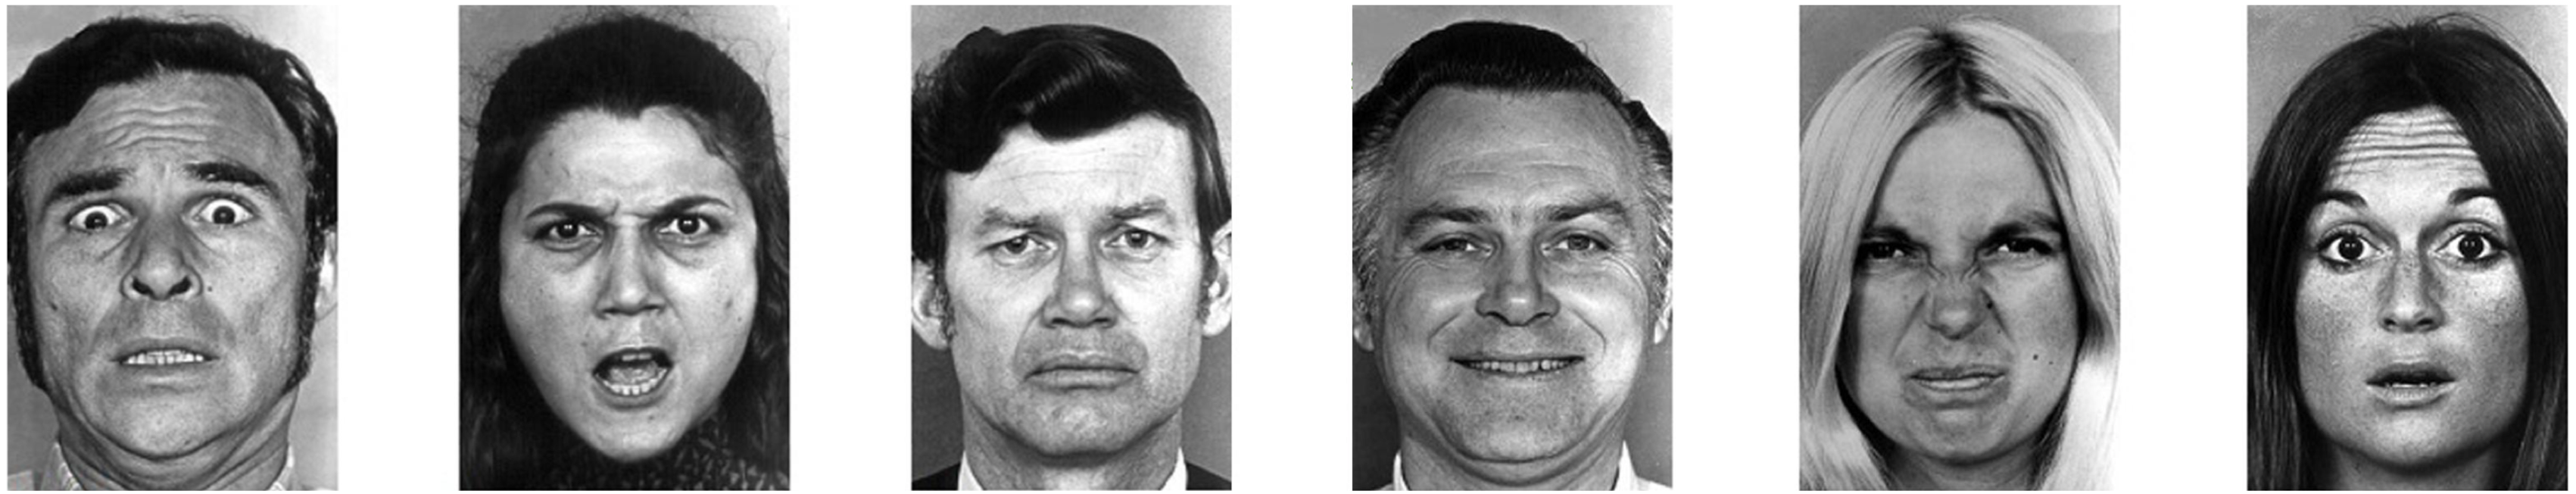
\includegraphics[width=\textwidth]{Images/emotions.png}
    \caption{Emociones universales propuestas por Paul Ekman (de izquierda a derecha: miedo, ira, tristeza, alegría, asco y sorpresa) \cite{Ekman}.}
    \label{fig:emotions}
\end{figure}

Paul Ekman, la principal autoridad de las expresiones faciales en el ámbito de la psicología, ha argumentado la existencia de seis emociones básicas  (ira, asco, miedo, alegría, tristeza y sorpresa) \cite{Ekman}, mostradas en la \autoref{fig:emotions}. Cada una de ellas tiene un conjunto de patrones únicos en el movimiento muscular facial. Estos patrones, así como su estudio detallado e identificación, posteriormente han sido integrados en un sistema de codificación facial (FACS) \cite{FACS}, el cual proporciona las técnicas necesarias para asociar los músculos del rostro a su espacio emocional correspondiente. De hecho, gran parte de los intentos de automatizar el reconocimiento de las expresiones faciales, capaces de ofrecer una identificación automática y en tiempo real a partir de un análisis tridimensional de la cara del sujeto, se basan en este sistema \cite{FaceReader}.

Por otro lado, en los últimos años, y gracias principalmente a la irrupción y al enorme progreso que ha experimentado el campo del aprendizaje profundo y automático en el ámbito del reconocimiento visual \cite{DeepLearning}, se han comenzado a desarrollar nuevas técnicas y métodos de identificación de las expresiones faciales. Este hecho, además, ha supuesto un nuevo punto de inflexión en este entorno dados los espectaculares resultados obtenidos gracias a la implementación de estos nuevos modelos, cuya eficacia y rendimiento se van a intentar analizar y reproducir en este proyecto.

Por último, cabe destacar que actualmente ninguno de los modelos anteriormente descritos pretende reconocer las emociones subyacentes (una sonrisa forzada, por ejemplo), centrándose la identificación tan solo en la expresión del rostro del sujeto en un instante determinado.

\section{Aprendizaje Automático}

El aprendizaje automático es una rama de la inteligencia artificial y puede definirse como un área de estudio que proporciona a las computadoras la capacidad de aprender, sin éstas estar explícitamente programadas \cite{MachineLearning}. De esta forma, mediante los variados algoritmos de aprendizaje automático es posible generar un resultado, generalmente un conjunto de predicciones o decisiones, a partir de diversos datos de entrada sin la necesidad de agregar nuevas líneas de código al sistema inicial.

En lo que respecta al proceso de aprendizaje del modelo en sí, es posible distinguir tres categorías por las que se rige este procedimiento y cuya clasificación está basada en el tipo o en la existencia de retroalimentación durante el entrenamiento:
\begin{itemize}
  \item \textbf{Aprendizaje supervisado}. Se caracteriza por la recepción de un conjunto de entradas etiquetadas, las cuales son atribuidas a la clase de pertenencia correspondiente gracias al algoritmo de aprendizaje pertinente. En este proceso de asignación el modelo va adaptándose o modificando sus parámetros con el fin de ofrecer un mejor rendimiento.
  \item \textbf{Aprendizaje no supervisado}. En este caso se recibe un conjunto de entradas sin etiquetar, por lo que el modelo intenta aprender de estos datos de entrada mediante la exploración de los patrones existentes en ellos.
  \item \textbf{Aprendizaje por refuerzo}. Se distingue por implementar un sistema de recompensa o castigo en función de las decisiones que un agente de \textit{software} ha tomado en un entorno dado para alcanzar un objetivo concreto.
\end{itemize}

Particularmente en este proyecto y tal y como se podrá comprobar durante los siguientes capítulos, el planteamiento del problema del reconocimiento de emociones desde el punto de vista de las herramientas y de los conjuntos de datos empleados en este trabajo implica un acercamiento hacia la utilización de técnicas de aprendizaje supervisado.

\subsection{Redes Neuronales Artificiales} \label{Chapter:ANN}

El aprendizaje supervisado tiene un conjunto de herramientas enfocadas a resolver problemas dentro de su dominio, siendo una de ellas, precisamente, las Redes Neuronales Artificiales (ANN).

\begin{figure}
    \centering
    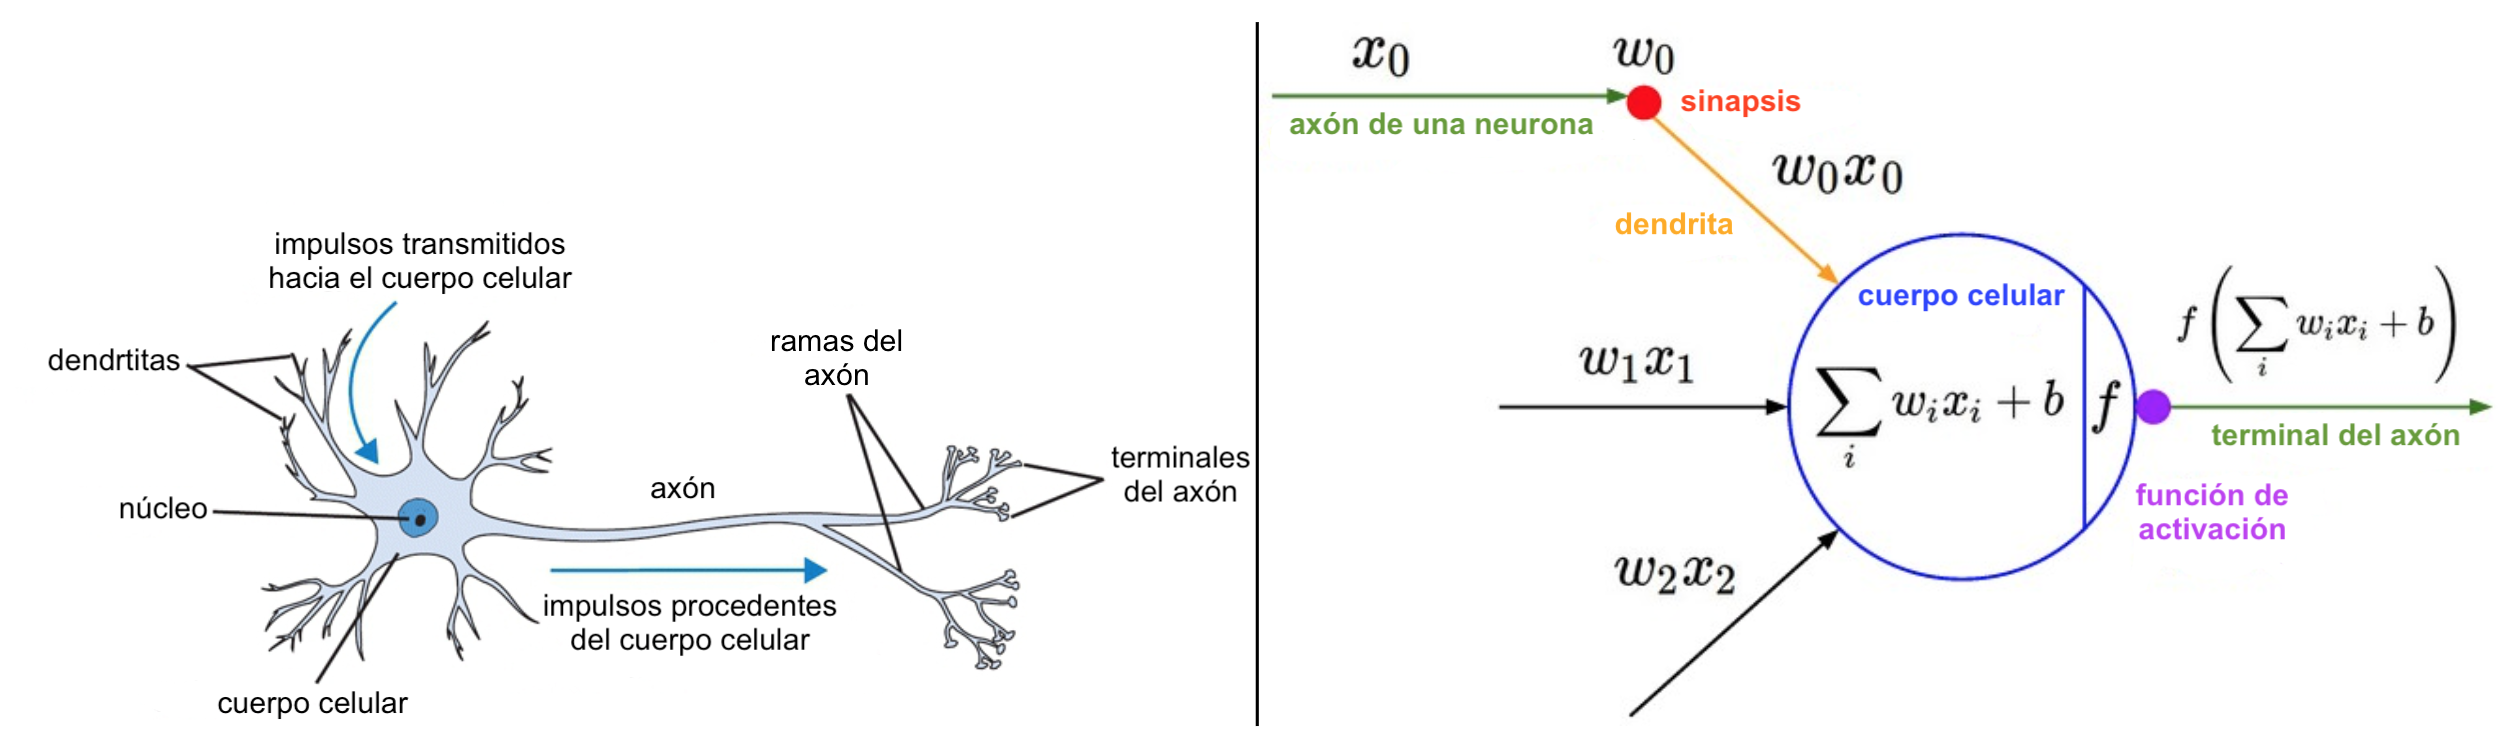
\includegraphics[width=\textwidth]{Images/analogy-neuron.png}
    \caption{Imagen de una neurona biológica (izquierda) y el modelo matemático que intenta reproducir superficialmente su funcionamiento (derecha) \cite{CS231n}.}
    \label{fig:analogy}
\end{figure}

Estas redes son un modelo computacional vagamente inspirado en las redes neuronales biológicas que constituyen los cerebros humanos \cite{ANN} y cuya analogía con el modelo matemático se puede observar en la \autoref{fig:analogy}. Cada una de estas neuronas recibe una serie de señales de entrada en sus dendritas y produce determinadas señales de salida que son trasladadas a lo largo del axón, el cual posteriormente se bifurca y se conecta a través de la sinapsis a las dendritas de otras neuronas. En el modelo computacional, por su parte, las señales que se desplazan a lo largo de los axones ($x_i$) interactúan de forma multiplicativa ($\omega_i\cdot x_i$) con las dendritas de otras neuronas en función de las fuerzas sinápticas (los pesos $\omega_i$), que son precisamente los elementos aprehensibles de los algoritmos de aprendizaje automático. Estos pesos, por lo tanto, son los que controlan la intensidad y la dirección (sinapsis excitatoria --peso positivo-- o inhibitoria --peso negativo--) de influencia de una neurona sobre otra. En el modelo biológico, las dendritas trasladan estas señales provenientes de otras neuronas al cuerpo celular, donde su suma da lugar a un potencial excitatorio postsináptico, que en caso de superar un determinado umbral causará la generación de un impulso eléctrico o potencial de acción que será enviado a largo del axón de la propia neurona. Este proceso en el modelo computacional es menos complejo al considerar que la información se encuentra tan sólo en la frecuencia de disparo del potencial de acción. En base a esta interpretación, la descarga de una neurona artificial se modela con una función de activación no lineal que representa la frecuencia de los impulsos a lo largo del axón, es decir, se toma como entrada la intensidad de la señal después de la suma ($\sum\limits_{i=0}^n \omega_i\cdot x_i + b$) y se normaliza, típicamente, según el tipo de función de activación, obteniéndose una salida acotada. Cabe destacar que el parámetro $b$, ignorado en los próximos capítulos por razones de simplificación, es necesario para evitar interrupciones en el proceso de aprendizaje cuando las entradas inyectadas ($x_i$) son nulas.

\begin{figure}
    \centering
    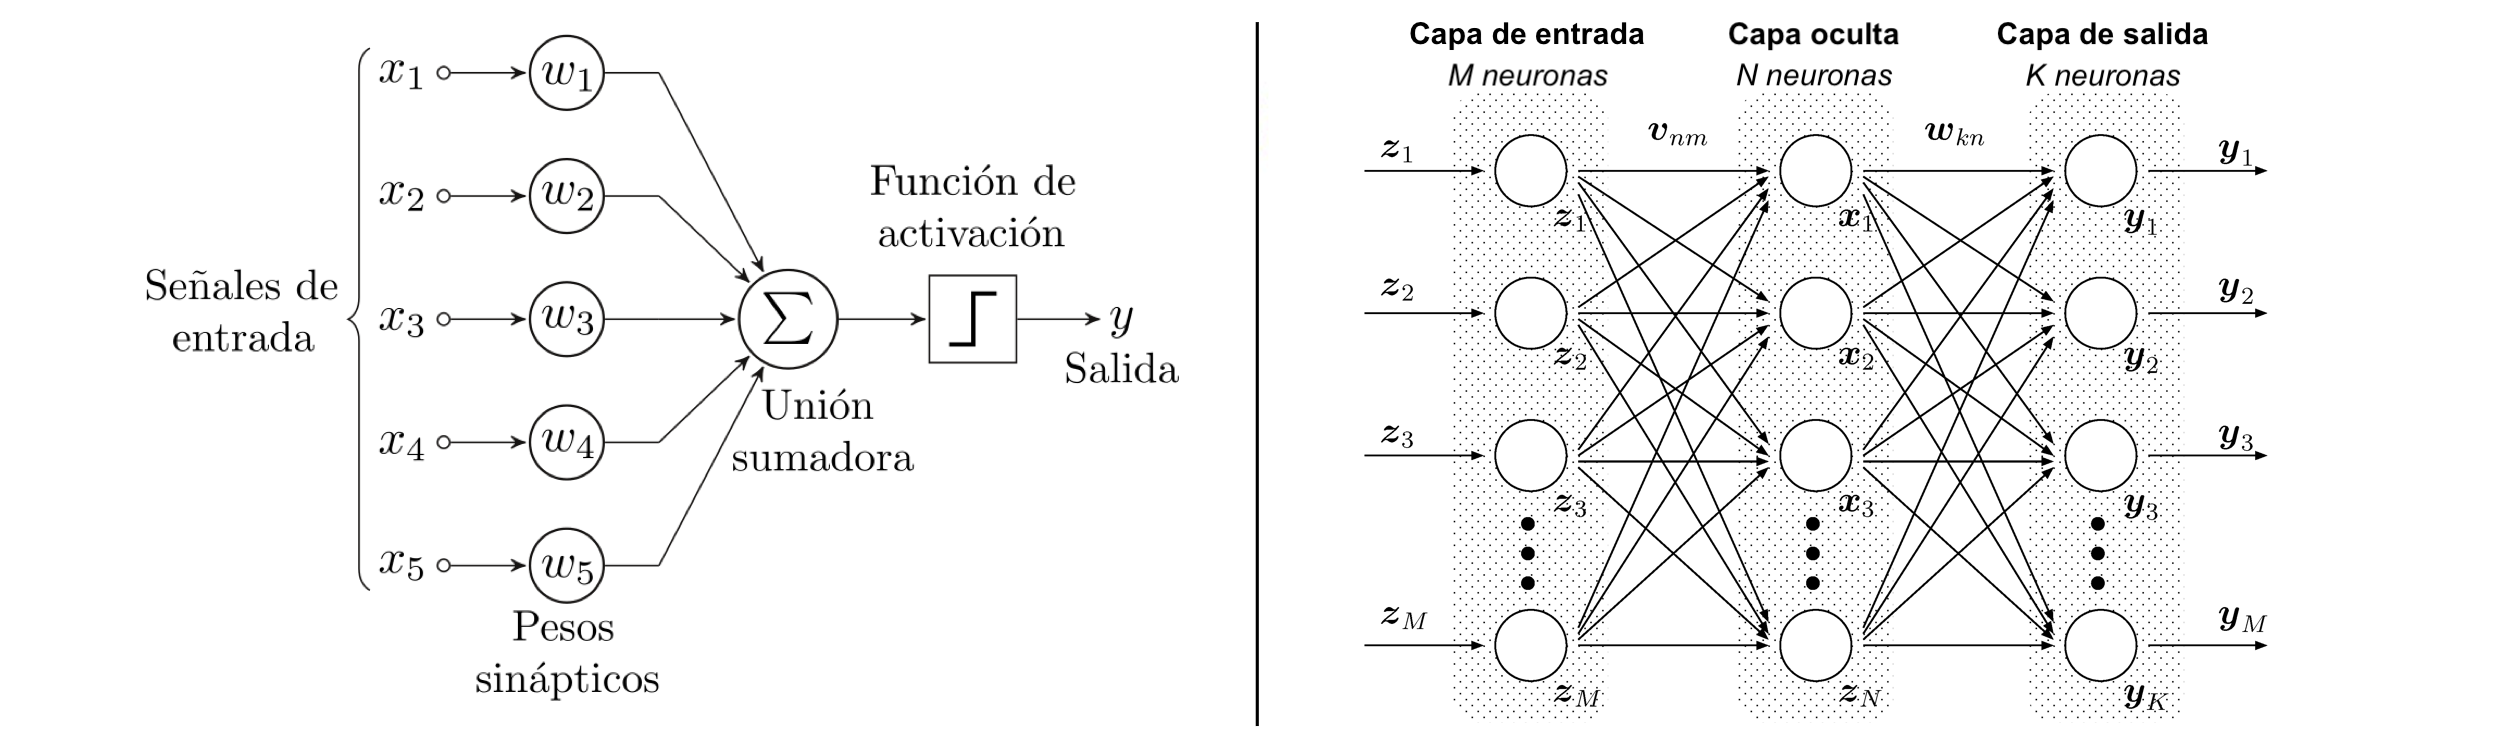
\includegraphics[width=\textwidth]{Images/perceptron_MLP.png}
    \caption{Topología de un perceptrón simple (izquierda) \cite{img:perceptron} y de un MLP con una capa oculta (derecha) \cite{img:MLP}.}
    \label{fig:ANN}
\end{figure}

Una ANN, por lo tanto, es una red estratificada de estas neuronas artificiales, pudiendo consistir en una capa de entrada, capas ocultas y una capa de salida \cite{Engelbrecht}. Las estructuras más básica de una ANN, el perceptrón y el perceptrón multicapa (MLP), que permite resolver problemas que no son linealmente separables, se representan en la \autoref{fig:ANN}.

En definitiva, una ANN es un conjunto de funciones que realizan una predicción que es expresada, generalmente, como una distribución de probabilidad para todas las etiquetas. Esta predicción, posteriormente, es cuantificada con respecto al valor real correspondiente, obteniéndose una función de error o de pérdidas, la cual es utilizada para actualizar los pesos de las distintas capas con el fin de mejorar la predicción global. Esto se lleva a cabo, tradicionalmente, mediante el método de propagación hacia atrás de errores o retropropagación y cuyas características se analizarán en profundidad en la \autoref{Chapter:Backpropagation}.

En cuanto al contexto histórico, las unidades neuronales fueron reconocidas por primera vez como elementos funcionales del sistema nervioso a finales del siglo XIX a través del trabajo de Santiago Ramón y Cajal. Mediante su estudio, gracias al cual obtuvo el Premio Nobel, propuso que estas células discretas interconectadas establecían una red compleja para la transmisión de la información. Esta descripción se conoce como la doctrina de la neurona y es el modelo aceptado a día de hoy en neurofisiología.

Posteriormente, estas redes, pese a formularse como un modelo para la realización de cálculos matemáticos en la década de los cuarenta \cite{McCulloch}, no fueron implementadas como tales hasta finales de los cincuenta, cuando fue presentada la arquitectura más simple de las ANN: el perceptrón \cite{Rosenblatt}. Este estaba formado por una serie de capas que contaban con un número determinado de nodos, cada uno de los cuales, excepto los de la entrada, representaban justamente a una neurona biológica. Además, fue en este artículo  en el que se introdujo precisamente la técnica de aprendizaje supervisado denominada retropropagación para entrenar las redes neuronales artificiales. 

A pesar de este gran paso, las limitaciones computacionales y de \textit{hardware} de la época (también existentes hoy en día), así como un enfoque de la investigación en inteligencia artificial hacia las representaciones simbólicas de los problemas, hizo que no fuera hasta principios de la década de los noventa cuando estas redes neuronales artificiales volvieran a cobrar protagonismo. Los responsables de ello fueron diversas publicaciones de una serie de modelos que explotaban las ANN, como la NETtalk \cite{NETtalk}, que mediante el aprendizaje automático fue capaz de aprender a leer en voz alta, o la ANN de múltiples capas desarrollada por Yann LeCun \cite{MNIST}, que permitía el reconocimiento de dígitos escritos a mano tomados de los códigos postales. Esta última publicación, de hecho, fue la pionera en integrar el reconocimiento de imágenes y el aprendizaje automático en un mismo modelo, además de introducir una serie de conceptos que posteriormente serían clave en el desarrollo de las Redes Neuronales Convolucionales (CNN), tales como la asignación de objetos según sus características a una serie de clases o la compartición de los pesos.

Cabe destacar que durante esta década muchos investigadores preferían utilizar las Máquinas de Vectores de Soporte (SVM) en las tareas de aprendizaje supervisado, cuya simplicidad y resultados eclipsaban a las ANN. Sin embargo, esta situación cambiaría drásticamente a partir del año 2010, cuando el desarrollo de potentes y asequibles herramientas de \textit{software} y de \textit{hardware}, junto con la existencia de una enorme cantidad de datos a explotar, posibilitaron la realización de cálculos extremadamente grandes sobre modelos complejos, obteniéndose unos resultados sin precedentes y que marcarían el auge del aprendizaje profundo.

\section{Aprendizaje Profundo}

El último resurgimiento de las ANN se conoce como aprendizaje profundo, término cuya definición puede englobarse en los siguientes puntos estrechamente relacionados \cite{def:DeepLearning}:
\begin{itemize}
  \item Es una clase de técnicas de aprendizaje automático que permite la explotación de un gran número de capas que procesan la información de forma no lineal para la extracción, transformación, análisis  y clasificación de patrones.
  \item Es un subcampo dentro del aprendizaje automático basado en algoritmos cuya función es aprender los múltiples niveles de representación de la información de la entrada con el fin de poder modelar relaciones complejas entre los datos en una arquitectura profunda, definiéndose los conceptos del nivel superior a partir de los del nivel inferior.
  \item Es una nueva área de investigación del aprendizaje automático introducida con el objetivo de acercar este subcampo de las ciencias de la computación a uno de sus objetivos originales: la inteligencia artificial. 
\end{itemize}

Estas técnicas y métodos que permiten aprender determinadas características por sí mismos a partir de representaciones sencillas han tenido un especial éxito en campos como la visión por computador, el procesamiento del lenguaje natural y el reconocimiento automático de voz. En el área del reconocimiento visual artificial, por ejemplo, una ANN puede alimentarse con los píxeles de una imagen, determinando posteriormente el algoritmo de aprendizaje si esta específica combinación representa cualquier característica particular que es repetida a través de una o varias imágenes.

Por otro lado, el hecho de que hoy en día ya no se emplee el término de ANN, sino el de aprendizaje profundo, se debe principalmente al impulso que recibió el campo de la inteligencia artificial gracias al trabajo de Geoffrey Hinton. Fue precisamente su publicación de 2012 sobre el reconocimiento automático de voz \cite{Hinton}, con la colaboración de los grupos de investigación de la Universidad de Toronto, Micrososft Research, Google Research e IBM Research, la primera que contenía una implementación directa en el ámbito industrial de las técnicas de aprendizaje profundo.

En lo que respecta al ámbito de la visión por computador, el punto crítico también llegaría de la mano de Hinton dentro del contexto del Desafío del Reconocimiento Visual a Gran Escala (ILSVRC) \cite{ILSVRC}. Esta competición consiste en evaluar el desempeño de los modelos de los participantes en la clasificación de 100\,000 fotografías etiquetadas a mano con la presencia o ausencia de 1\,000 categorías de objetos diferentes. Su creación en 2010, así como de la base de datos ImageNet utilizada para el entrenamiento, tenían como objetivo motivar la investigación de \textit{software} enfocado al campo del reconocimiento visual. De hecho, el avance experimentado tan sólo dos años después de la aparición del ILSVRC es considerado ampliamente como el comienzo de la revolución del aprendizaje profundo, tanto en el entorno de investigación de la inteligencia artificial como en el de la industria tecnológica \cite{AIboom}. Este progreso estuvo marcado por la presentación, por parte de Alex Krizhevsky, Ilya Sutskever y Geoffrey Hinton, de un modelo capaz de reducir a la mitad la tasa de error existente en ese momento \cite{Krizhevsky}. El sistema desarrollado combinaba varios elementos críticos que se convertirían en los pilares fundamentales de los modelos de aprendizaje profundo: el entrenamiento mediante las Unidades de Procesamiento Gráfico (GPUs), las Redes Neuronales Convolucionales (CNN), el empleo de la Unidad Lineal Rectificada (ReLU) y del método para evitar el sobreentrenamiento, conocido como \textit{dropout}.

\subsection{Empleo de las Unidades de Procesamiento Gráfico}

Probablemente el componente más relevante e influyente dentro del explosivo progreso del aprendizaje profundo haya sido el uso de las Unidades de Procesamiento Gráfico en el entrenamiento de los modelos diseñados.

\begin{figure}
    \centering
    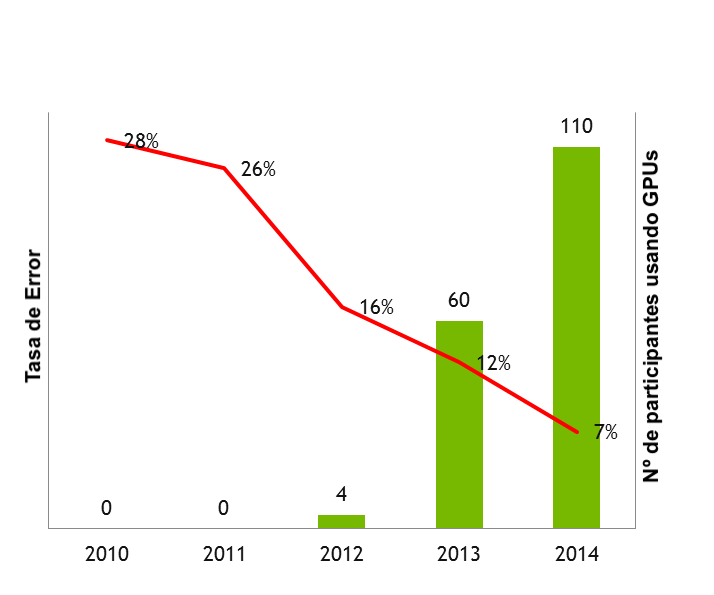
\includegraphics[scale=0.8]{Images/ILSVRC.png}
    \caption{Tasa de error de la entrada ganadora del ILSVRC (línea roja) y número creciente de entradas que usan GPUs cada año (barras verdes).\cite{img:ILSVRC}}
    \label{fig:ILSVRC}
\end{figure}

Las GPUs son esencialmente calculadoras de coma flotante cuya arquitectura paralela de miles de núcleos ofrece la posibilidad de manejar múltiples tareas simultáneamente. Esta capacidad de paralelización, precisamente, es la que ha sido ampliamente explotada por los algoritmos de aprendizaje profundo en la realización de operaciones vectoriales y matriciales, logrando una reducción de los tiempos de entrenamiento en unas 10 -- 20 veces \cite{DeepLearning}. Esto ha posibilitado, a su vez, el entrenamiento de modelos significativamente más complejos o profundos y por lo tanto, la obtención de tasas de error cada vez más bajas.

El desarrollo experimentado y su influencia pueden apreciarse en la \autoref{fig:ILSVRC}, que muestra como los resultados del ILSVRC van mejorando a medida que se populariza el uso de las GPUs. Destaca también la caída precipitada del año 2012 propiciada por la implementación de la red AlexNet, modelo que se ha descrito brevemente en el apartado anterior y que ha revolucionado el reconocimiento e identificación visual, siendo especialmente relevante en este proyecto.

\section{Redes Neuronales Convolucionales} \label{Chapter:CNN}

Las investigaciones sobre la corteza visual animal, cuyos primeros estudios trascendentales datan de 1968 con la publicación de Hubel y Wiesel sobre los campos receptivos y la arquitectura funcional del córtex visual de los monos \cite{Hubel}, están estrechamente relacionadas con el desarrollo de las redes neuronales convolucionales. Fue precisamente en este estudio en el que se describió por primera vez cómo las señales obtenidas por los ojos son procesadas por parcelas visuales en el neocórtex para generar detectores de bordes, de movimientos, de profundidad y de color, construyendo bloques de la escena visual.

Una de las primeras implementaciones inspiradas en este estudio fue el Neocognitron \cite{Neocognitron}. Este modelo de red neuronal intentaba imitar el funcionamiento de los dos tipos de células introducidas en el anterior documento: las células simples, que responden principalmente a bordes y a líneas de orientaciones particulares y las células complejas, que presentaban campos receptivos más grande e invariancia local. A pesar de todo ello, este modelo presentaba un importante inconveniente en el proceso de aprendizaje al no haberse desarrollado, por aquella época, un método para ajustar los valores de los pesos con respecto a una medida de error para toda la red, como la retropropagación. Esta técnica de propagación hacia atrás de errores, analizada en \autoref{Chapter:Backpropagation}, no fue implementada en el entrenamiento de las ANN hasta 1985, cuando se publicó el trabajo de Rumelhart, Hinton y Williams \cite{Rumelhart}.

A partir de este momento se llevaron a cabo numerosas implementaciones con aplicaciones prácticas empleando la propagación hacia atrás de errores para entrenar las CNN, siendo Yann LeCun con su clasificador de dígitos escritos a mano (MNIST) \cite{MNIST} el pionero e inspirando, además, gran parte de las investigaciones futuras.

En cuanto a las redes neuronales convolucionales en sí, éstas son muy similares a las redes neuronales ordinarias tratadas en la \autoref{Chapter:ANN}: están formadas por neuronas que tienen pesos que se pueden aprender, reciben entradas a las que se aplica un producto escalar y opcionalmente una función no lineal, y obtienen, en la última capa, la puntuación de pertenencia a una determinada clase. La principal diferencia, por lo tanto, es que las arquitecturas convolucionales suponen explícitamente que las entradas son imágenes, haciendo que las operaciones sean más eficientes y reduciendo inmensamente la cantidad de parámetros en la red \cite{CS231n}. Además, las capas de una CNN tienen neuronas dispuestas en las 3 dimensiones: anchura, altura y profundidad, volumen que coincide, precisamente, con las dimensiones en píxeles (ancho y alto) y el modelo de color (profundidad), tradicionalmente RGB, de una imagen. Asimismo, las neuronas de una determinada capa de una CNN sólo están conectadas a una pequeña región de la capa anterior, en lugar de a todas las neuronas de una manera absolutamente conectada, como ocurría en las ANN. Es por ello que al final de la arquitectura de una CNN la imagen completa de la entrada se reduce a tan solo un vector de puntuaciones de pertenencia a una determinada clase dispuesto a lo largo largo de la dimensión de profundidad, tal y como se puede observar en la \autoref{fig:CNN}.

\begin{figure}
    \centering
    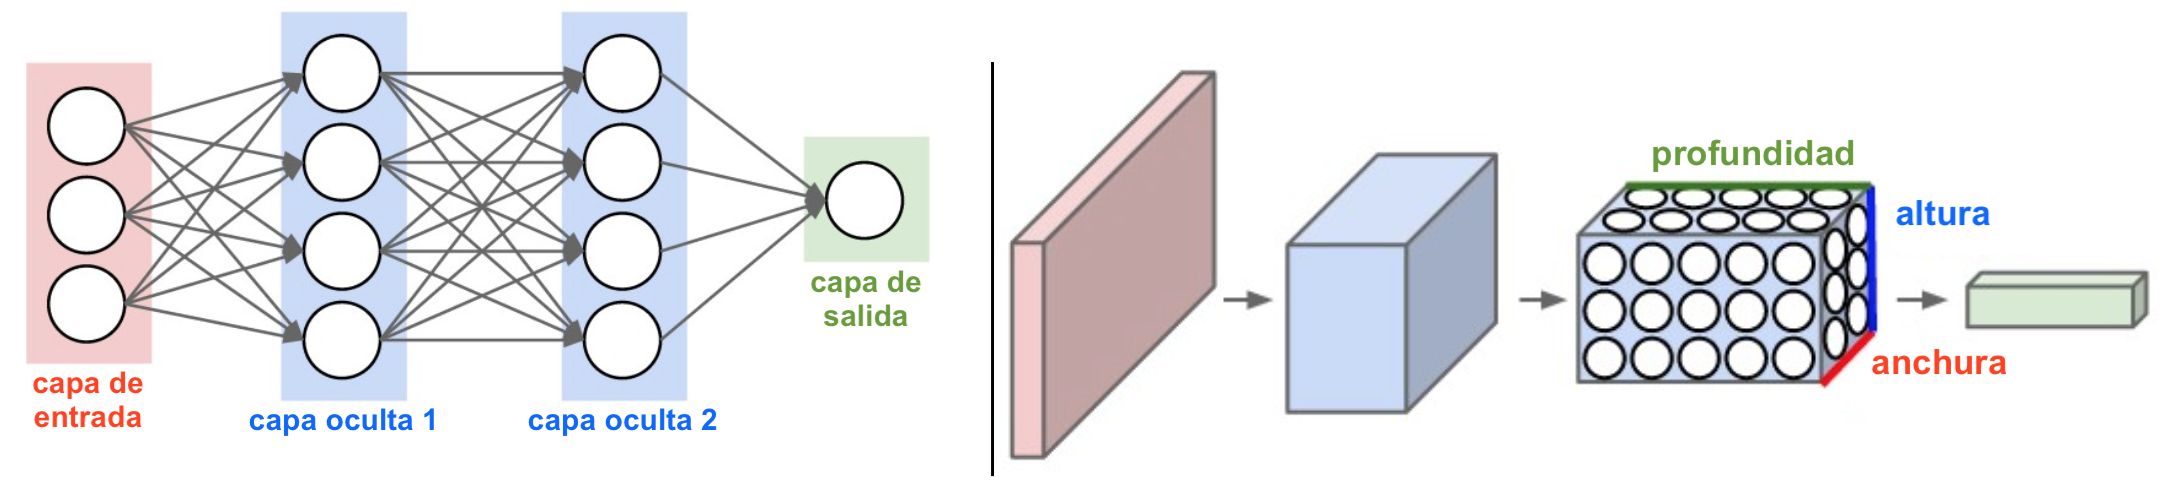
\includegraphics[width=\textwidth]{Images/CNN.png}
    \caption{Una ANN ordinaria de 3 capas (izquierda) y una CNN (derecha) \cite{CS231n}.}
    \label{fig:CNN}
\end{figure}

En definitiva, una CNN simple es una secuencia de capas que se encargan de transformar un volumen de activación en otro diferente a través de una función diferenciable. Generalmente, y particularmente en este proyecto, son utilizadas principalmente las capas descritas en \autoref{Chapter:Layers} (capas convolucionales, de agrupación o \textit{pooling}, íntegramente conectadas, etc.), con cuyo apilamiento sucesivo se va a pretender formar una arquitectura neuronal convolucional completa.

Algunas de estas arquitecturas, especialmente las más relevantes en el contexto de este proyecto, se enumeran a continuación:
\begin{itemize}
  \item \textbf{LeNet} \cite{LeNet-5}. Las primeras aplicaciones exitosas de las CNN fueron desarrolladas por Yann LeCun en la década de 1990. Entre ellas, la más conocida es la arquitectura LeNet, que se utilizó para leer los dígitos de los códigos postales.
  \item \textbf{AlexNet} \cite{Krizhevsky}. La publicación con la que se popularizó el uso de las CNN en el campo de la visión por computador fue la ya nombrada anteriormente AlexNet. Este modelo se presentó al desafío ILSVRC de ImageNet en 2012, superando al segundo finalista con una diferencia de más del 10\% en la tasa de error. En cuanto a su arquitectura, era muy similar a LeNet, con la diferencia de que presentaba capas convolucionales más profundas, más grandes y apiladas unas sobre otras, cuando lo común era tener capas convolucionales seguidas inmediatamente de capas de agrupación.
  \item \textbf{GoogLeNet} \cite{GoogleNet}. El ganador del ILSVRC 2014 fue una CNN desarrollada por el grupo de investigación de inteligencia artificial de Google. Su principal contribución fue la introducción de un modelo con el que se consiguió reducir drásticamente la cantidad de parámetros en la red, pasando a contar con tan sólo 4 millones, un número más que razonable teniendo en cuenta los 60 millones de la red AlexNet. También cabe destacar las posteriores versiones de GoogLeNet desarrolladas, como Inception-v3 e Inception-v4, que, como se verá en el \autoref{Chapter:5}, son fundamentales en el presente proyecto.
  \item \textbf{VGGNet} \cite{VGGNet}. Obtuvo el segundo puesto en el desafío ILSVRC 2014, aportando y desarrollando la idea de que la profundidad de la red es un componente crítico para la obtención de buenos resultados. Sin embargo, a pesar de  haber alcanzado una tasa de error más que razonable, este modelo presentaba una importante desventaja al contar con casi 140 millones de parámetros, haciéndolo muy costoso de entrenar y requiriendo, además, mucha memoria.
  \item \textbf{ResNet} \cite{ResNet}. Esta red residual fue la vencedora del ILSVRC 2015 al implementar una serie de conceptos clave como las conexiones directas entre capas no contiguas y la normalización por lotes, lo que además de acelerar la evaluación del modelo, favorecía la prevención del sobreaprendizaje. Actualmente, de hecho, las ResNet o sus variaciones son la opción predeterminada para implementar las CNN en la práctica \cite{ImpactResNet}.
\end{itemize}

\subsection{Retropropagación} \label{Chapter:Backpropagation}

\begin{figure}
    \centering
    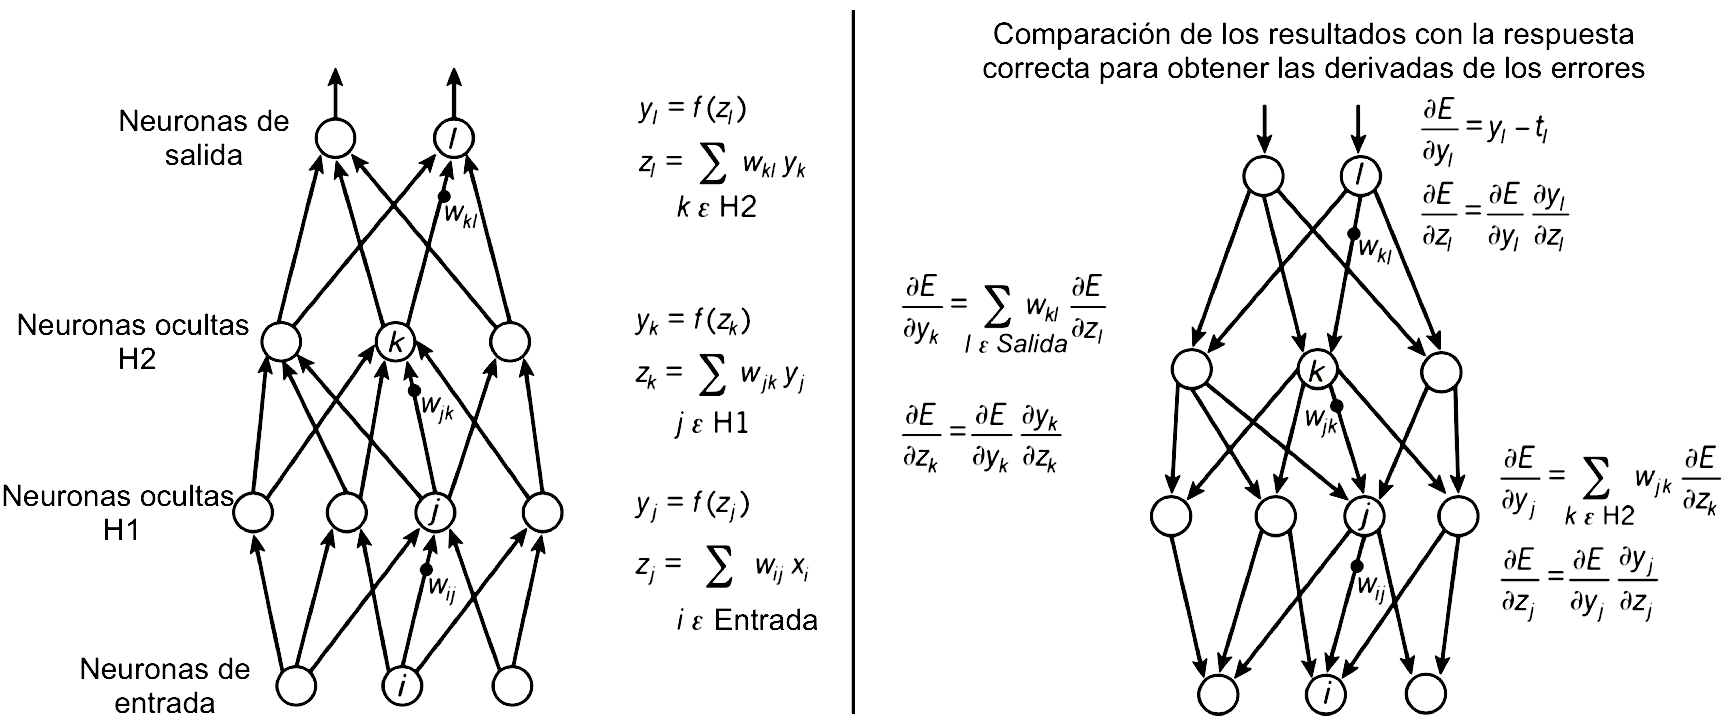
\includegraphics[width=\textwidth]{Images/backpropagation.png}
    \caption{Ecuaciones utilizadas para calcular las salidas o predicciones de una red neuronal con dos capas ocultas y una capa de salida (izquierda) y las ecuaciones empleadas en la retropropagación si la función de pérdidas para cada una de las unidades neuronales es $\frac{1}{2}\cdot (y_l - t_l)^2$, donde $t_l$ es el valor objetivo (derecha) \cite{DeepLearning}.}
    \label{fig:backpropagation}
\end{figure}

El procedimiento de la retropropagación para calcular el gradiente de una función de pérdidas con respecto a los pesos, posteriormente actualizados, de una serie de módulos multicapa no es más que una aplicación práctica y recursiva de la regla de la cadena para derivadas \cite{DeepLearning}. La idea clave es que el gradiente de la función objetivo con respecto a la entrada se calcula en la salida y se distribuye hacia atrás a través de las distintas capas de la red, tal y como puede apreciarse en la \autoref{fig:backpropagation}. De esta manera, la ecuación de la retropropagación puede aplicarse repetidamente para propagar los gradientes a través de todos los módulos, desde la parte superior, donde la red genera una predicción determinada, hasta la parte inferior, donde es alimentada la entrada con datos externos. Esta propagación, sin embargo, no es uniforme, sino que cada una de las neuronas de las capas ocultas tan sólo recibe una fracción de la señal total de error correspondiente a la contribución relativa que aporta a la salida original. Posteriormente, una vez que estos gradientes analíticos se calculan, son utilizados para realizar una actualización de los parámetros de la red mediante un optimizador. Hay numerosos enfoques para realizar esta actualización, discutidos en la \autoref{Chapter:Optimizers}.

El pseudocódigo completo de este proceso se explica detalladamente en el \autoref{alg:Backpropagation} del \autoref{Appendix:Algorithms}.

\subsection{Actualización de parámetros} \label{Chapter:Optimizers}

Actualmente, los dos métodos más empleados y recomendados para realizar la actualización de parámetros, con el objetivo de encontrar una serie de pesos $\omega_{i,j}$ que minimicen la función de pérdidas, son el Descenso Estocástico del Gradiente (SGD) con Nesterov Momentum y la Estimación del Momento Adaptativo (Adam) \cite{CS231n}.

\subsubsection{Descenso Estocástico del Gradiente con Nesterov Momentum}

La forma más simple y común de llevar a cabo la optimización es, precisamente, mediante SGD, que permite modificar los parámetros en la dirección negativa del gradiente (\autoref{eq:SGD}), al apuntar éste en la dirección del máximo en cada uno de los puntos evaluados, con el fin de minimizar la función de pérdidas.
\begin{align} \label{eq:SGD}
    \omega_t &= \omega_{t-1} - \lambda \cdot \nabla f(\omega_{t-1}) \\
    \text{donde}~  
    \omega_t &\equiv \text{peso en un instante determinado,} \notag \\
    \lambda &> 0 \text{\space es la tasa de aprendizaje} \notag
\end{align}
Los métodos Momentum, por su parte, presentan un enfoque que ofrece mejores tasas de convergencia, ya que emplean el gradiente para actualizar los parámetros de una forma más efectiva al acumular velocidad en las direcciones que reducen continuamente la función de pérdidas, tal y como se muestra en la \autoref{eq:SGDMomentum}. 
\begin{align}
    v_t &= \mu \cdot v_{t-1} - \lambda \cdot \nabla f(\omega_{t-1}) \\
    \omega_t &= \omega_{t-1} + v_t \label{eq:SGDMomentum} \\ 
    \text{donde}~
    v &\equiv \text{ vector de velocidad,} \notag \\
    \mu &\in [0,1] \text{\space es el momento lineal} \notag
\end{align}
\begin{figure}
    \centering
    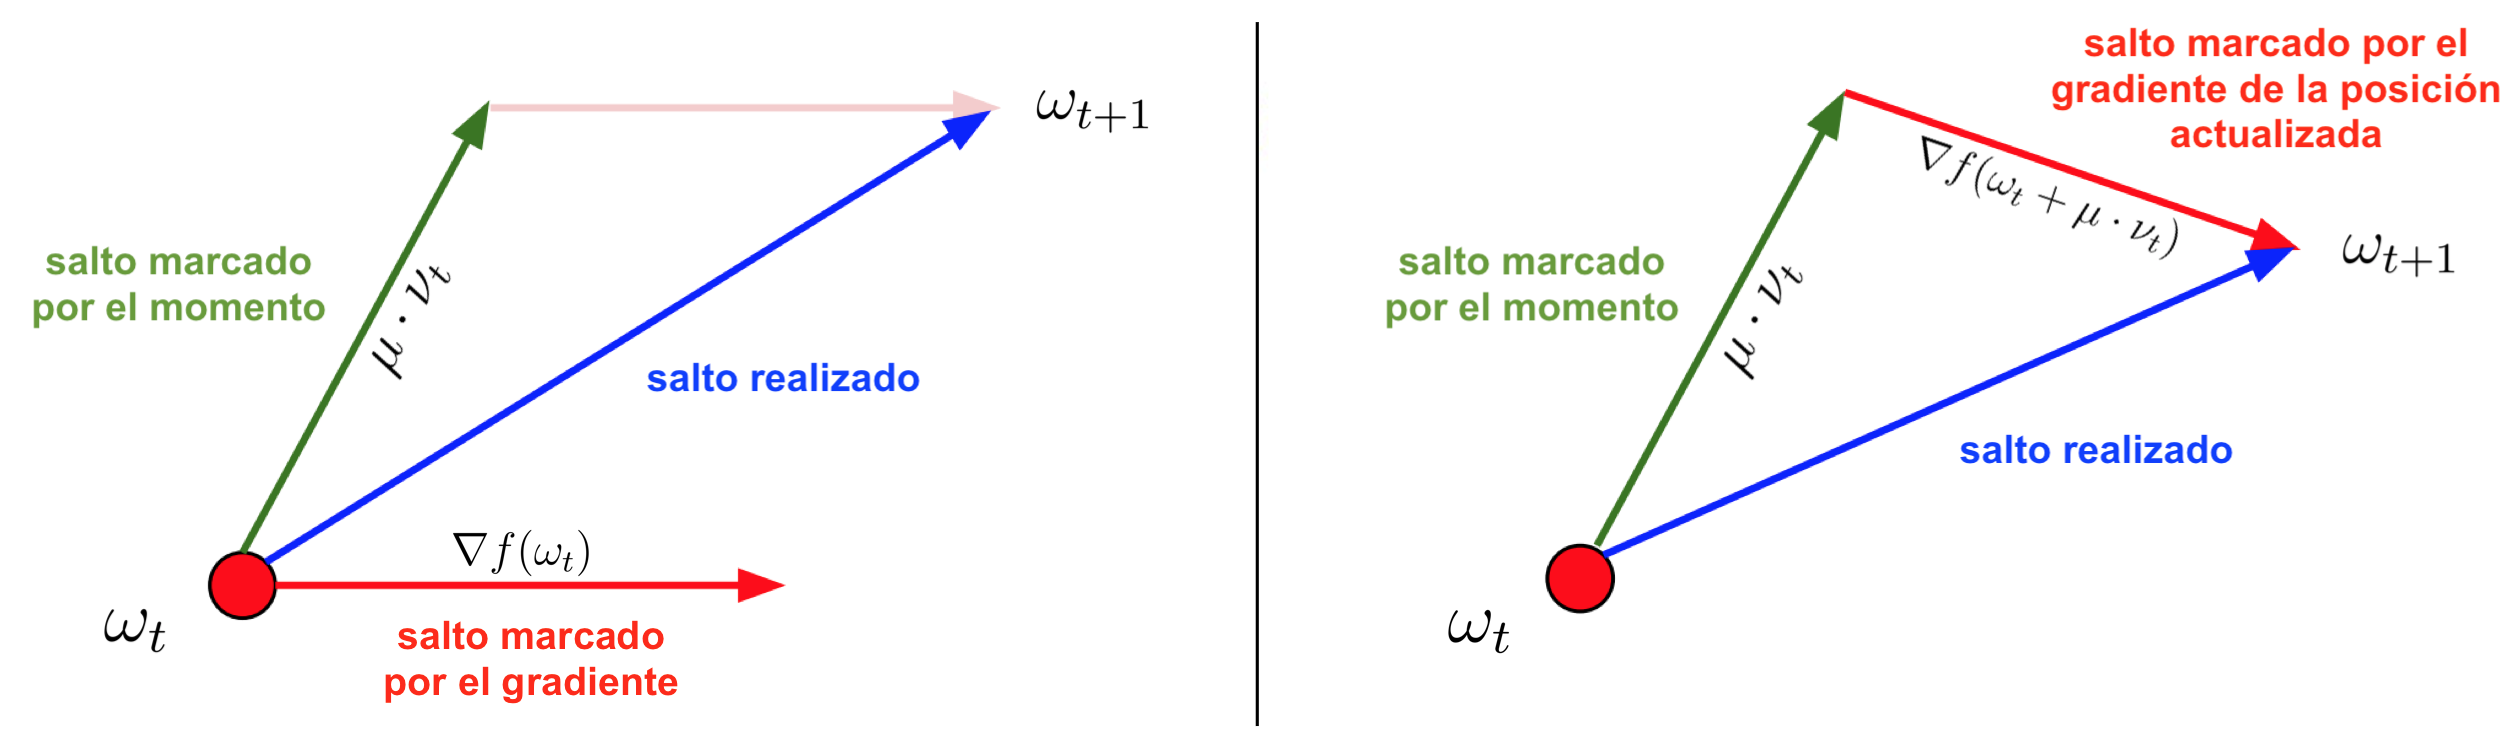
\includegraphics[width=\textwidth]{Images/NesterovMomentum.png}
    \caption{Actualización Momentum (izquierda) y actualización Nesterov Momentum (derecha) \cite{CS231n}.}
    \label{fig:NesterovMomentum}
\end{figure}

Nesterov Momentum, a su vez, también goza de mayores garantías teóricas de convergencia, funcionando ligeramente mejor en la práctica que el método Momentum estándar \cite{Sutskever}. En la \autoref{fig:NesterovMomentum} se puede observar la comparación, haciéndose evidente el aumento de la eficacia de este último procedimiento representado mediante la \autoref{eq:SGDNesterovMomentum}, que da primero los saltos en la dirección del gradiente acumulado anterior para posteriormente calcular el gradiente en la posición actualizada y realizar una corrección.
\begin{align} 
    v_t &= \mu \cdot v_{t-1} - \lambda \cdot \nabla f(\overbrace{\omega_{t-1} + \mu \cdot v_{t-1}}^{w_{salto}}) \\
    \overbrace{\omega_t}^{w_{corregido}} &= \omega_{t-1} + v_t \label{eq:SGDNesterovMomentum}
\end{align}

\subsubsection{Estimación del Momento Adaptativo}

Al contrario que el método del descenso estocástico del gradiente, que permite manipular la tasa de aprendizaje de forma global e idéntica para toda la red, Adam adapta la tasa de aprendizaje a cada uno de los parámetros presentes en el modelo. En el artículo que describe este algoritmo, los autores exponen a Adam como la combinación de dos de las extensiones de SGD \cite{Adam}:
\begin{itemize}
  \item Algoritmo de \textbf{Gradiente Adaptativo (AdaGrad)}, el cual presenta una tasa de aprendizaje adaptativa por parámetro que mejora el rendimiento de sistemas con gradientes dispersos, como es el caso de los problemas de visión por computador. 
  \item \textbf{Propagación del Valor Cuadrático Medio (RMSProp)}, que también explota las tasas de aprendizaje adaptativas, basadas en este caso en el promedio de las magnitudes recientes de los gradientes, lo que proporciona buenos resultados para problemas ruidosos. 
\end{itemize}

De esta forma, Adam, además de almacenar un promedio del primer momento (la media), como en RMSProp, también utiliza el promedio de los segundos momentos de los gradientes (la varianza) para la actualización de los parámetros, proceso que se rige por la \autoref{eq:Adam}.
\begin{align}
    m_t &= \beta_1 \cdot m_{t-1} + (1 - \beta_1) \cdot \nabla f(\omega_{t-1}) \\
    v_t &= \beta_2 \cdot v_{t-1} + (1 - \beta_2) \cdot \nabla^2 f(\omega_{t-1}) \\
    \hat{m}_t &= m_t / (1 - \beta_1^t) \\
    \hat{v}_t &= v_t / (1 - \beta_2^t) \\
    \omega_t &= \omega_{t-1} - \lambda \cdot \hat{m}_t / (\sqrt{\hat{v}_t} + \epsilon) \label{eq:Adam} \\
    \text{donde}~
    \lambda &> 0 \text{\space es la tasa de aprendizaje,} \notag \\
    m_t \text{\space y \space} v_t &\equiv \text{estimaciones del primer y segundo momento,} \notag \\
    \hat{m}_t \text{\space y \space} \hat{v}_t &\equiv \text{estimaciones del primer y segundo momento corregidas} \notag
\end{align}
De forma específica, este algoritmo englobado en la \autoref{eq:Adam} calcula en un primer momento un promedio exponencial del gradiente ($m_t$) y del gradiente cuadrado ($v_t$), cuyas tasas de descenso son controladas mediante los parámetros $\beta_1$ y $\beta_2$. Por otro lado, como $m_t$ y $v_t$ son inicialmente nulos, es necesario aplicarles una corrección para evitar su sesgado hacia cero, especialmente notable durante las primeras iteraciones. Tras ello, se realiza la actualización de los parámetros de manera análoga al método del descenso estocástico del gradiente.

\section{Trabajos Relacionados} \label{Chapter:RelatedWork}

La tarea del reconocimiento de expresiones faciales puede abordarse desde múltiples puntos de vista, abarcando áreas como el procesamiento de señales, la visión por computador o el aprendizaje automático. Precisamente la combinación de estas técnicas es la que ofrece el entorno idóneo para el desarrollo e implementación de los sistemas de identificación de emociones.

En estas circunstancias, es destacable la labor del grupo de investigación comercial Affectiva, que es el líder mundial en reconocimiento de emociones. Su metodología se basa en técnicas de aprendizaje profundo aplicadas a la detección y seguimiento de rostros, a la transcripción de conversaciones, a la detección de la voz y a la clasificación de las emociones a partir de las expresiones faciales y del habla. Además, cabe destacar que los servicios ofrecidos por esta compañía son independientes de factores culturales o regionales dada la extensión de sus bases de datos \cite{Affectiva}, contando, por ejemplo, con casi 6 millones de representaciones faciales de 75 países diferentes. Este número es extraordinariamente elevado teniendo en cuenta que la mayoría de los conjuntos de entrenamiento públicos ni si quiera alcanzan las 5\,0000 imágenes.

En lo que respecta a un enfoque más similar a lo desarrollado en este escrito, tanto por el uso de la misma base de datos (FER-2013 \cite{FER-2013}, analizada en profundidad en la \autoref{Chapter:FER-2013}) como por la metodología empleada, es necesario señalar las siguientes implementaciones:
\begin{itemize}
  \item \textbf{Reconocimiento de Expresión Faciales utilizando Redes Neuronales Convolucionales: Estado del Arte \cite{Pramerdorfer}}. Este modelo, que actualmente está reconocido como el estado del arte en el ámbito del desafío FER-2013, es el resultado de la superación de una serie de cuellos de botella de los sistemas convolucionales (irregularidad de los datos, profundidad de la red, etc.). Su arquitectura está formada por un conjunto de CNNs ensambladas y basadas en modelos actuales y profundos (VGG, Inception y ResNet), así como por una serie de módulos de preprocesamiento que extraen distintos puntos de referencia de interés, igualan el histograma o realizan ajustes lineales a los datos de entrada. La precisión alcanzada por este sistema sobre el conjunto de evaluación de la base de datos FER-2013, sin otros entrenamientos auxiliares anteriores, ha sido de 75.20\%.
  \item \textbf{Aprendiendo los Rasgos de las Relaciones Sociales a partir de Imágenes Faciales \cite{Zhang}}. El modelo aquí descrito desarrolla una serie de técnicas de clasificación y extracción de características basadas en una CNN convencional y una capa adicional y paralela al modelo cuya influencia recae únicamente en la capa de decisión. Mediante esta implementación tan peculiar se pretende fusionar los datos de múltiples fuentes y conseguir, de esta forma, una aproximación espacial de las representaciones de los rostros aprendidos de clases afines. El rendimiento obtenido fue de 75.10\%.
  \item \textbf{Aprendizaje Profundo utilizando Máquinas de Vector de Soporte \cite{DeepSVM}}. El sistema presentado en este documento fue precisamente el ganador del desafío de reconocimiento de expresiones faciales (FER-2013) con una tasa de acierto de 71.16\%. Se caracteriza principalmente por combinar las redes neuronales y las SVM, minimizando, por lo tanto, una función de pérdidas basada en los márgenes de decisión en lugar de la entropía cruzada.
  \item \textbf{Clasificación de Emociones con Aumento de Datos mediante Redes Generativas Antagónicas \cite{GANAugmentation}}. La técnica propuesta en este artículo surge como resultado del estancamiento de los avances en el reconocimiento de expresiones faciales debido a las limitaciones de las bases de datos públicas existentes. Por ello, para complementar el conjunto de entrenamiento se ha propuesto una Red Generativa Antagónica de Ciclo Consecuente (CycleGAN) \cite{cycleGAN} con la que se consigue aumentar la variedad de datos, así como los márgenes entre clases semejantes. Los resultados empíricos han mostrado que es posible obtener un aumento de entre el 5\% y el 10\% en la tasa de acierto empleando estas técnicas.
  \item \textbf{Redes Neuronales Convolucionales para la Clasificación de Emociones y Género en Tiempo Real \cite{Arriaga}}. En este documento se expone un marco de implementación consistente en una red neuronal convolucional que realiza las tareas de detección de rostros, clasificación de género y predicción de emociones en tiempo real. La red propuesta está inspirada en la arquitectura Xception \cite{Xception}, que combina módulos convolucionales separables en profundidad y módulos residuales. La precisión obtenida sobre el conjunto de evaluación de expresiones faciales FER-2013 ha sido de 66\%.
\end{itemize}

Como puede observarse, dada la estandarización de la evaluación de todos estos modelos debido a las características de la base de datos empleada, dividida en tres subconjuntos (entrenamiento, validación y evaluación), los resultados que se van a presentar a lo largo de este proyecto van a poder compararse de forma directa con las tasas anteriormente mencionadas.
    \renewcommand{\tablename}{Tabla}
\chapter{Marcos de Implementación} \label{Chapter:3}

Actualmente hay una gran cantidad de entornos de trabajo desarrollados exclusivamente para el aprendizaje profundo. Algunos de los más populares son TensorFlow, Theano, Caffe, Keras o PyTorch. En el caso particular de este proyecto y tal como se expondrá a lo largo de este capítulo son usados básicamente dos: Keras y Tensorflow, dado que son los más versátiles al ofrecer la mayor cantidad de herramientas que simplifican notablemente las implementaciones y los que permiten una integración más directa con otras plataformas como Google Cloud u OpenCV.

También cabe mencionar que cada uno de estos entornos emplea el lenguaje de programación interpretado Python como interfaz de programación \textit{front end}, lo que lo convierte en el escenario mas extendido para el desarrollo de aplicaciones de aprendizaje automático. Además, Python es capaz de combinarse con lenguajes de programación de bajo nivel como C o C\texttt{++}, que actúan generalmente como \textit{back end}.

\section{Keras y TensorFlow}

Keras es una Interfaz de Programación de Aplicaciones (API) de redes neuronales de alto nivel, escrita en Python y capaz de ejecutarse sobre TensorFlow. Esta última, por su parte, es una biblioteca de software de código abierto desarrollada por el departamento de inteligencia artificial de Google para la computación numérica de alto rendimiento con la capacidad de implementarse y ejecutarse utilizando múltiples Unidades de Procesamiento Central (CPUs), Unidades de Procesamiento Gráfico (GPUs) y Unidades de Procesamiento Tensorial (TPUs).

La decisión del empleo de estas dos herramientas, concretamente de Keras sobre TensorFlow, radica en que su combinación proporciona un entorno modular, extensible y fácil de usar, ofreciendo un gran número de utensilios de aprendizaje profundo. En este contexto, Keras facilita tanto las herramientas para desarrollar las arquitecturas neuronales, como el medio y los métodos para entrenar los modelos. Además, en lo que respecta al campo del reconocimiento visual, pone a disposición de la comunidad una gran variedad de modelos preentrenados con distintas bases de datos y que pueden emplearse para la predicción, la extracción de características y la afinación de otros sistemas que planteen problemas similares. De hecho, la existencia de estos modelos, que son reconocidos como los estados del arte dentro de su ámbito, simplifica notablemente la implementación de técnicas como la transferencia de aprendizaje, tratada en el \autoref{Chapter:TransferLearning}.

\section{Google Cloud Plataform}

Google Cloud Platform es una plataforma que ofrece un conjunto de servicios modulares de computación en la nube, entre los que destacan el almacenamiento de datos, el análisis de datos y el aprendizaje automático. Dentro de este último punto, se van a utilizar básicamente tres herramientas: \begin{itemize}
  \item \textbf{Cloud Machine Learning Engine}. Es un servicio que proporciona un entorno de implementación de modelos complejos de aprendizaje automático, permitiendo ejecutar aplicación desarrolladas sobre TensorFlow con ciertas alteraciones. Concretamente, mediante este servicio es posible realizar tareas previas de procesado de datos, entrenar modelos de aprendizaje profundo y evaluar sistemas existentes.
  
  La GPU empleada por este servicio y la única ofrecida actualmente es la NVIDIA Tesla K80.
  \item \textbf{Compute Engine -- Cloud Datalab}. Este producto permite desarrollar proyectos en máquinas virtuales escalables de alto rendimiento y ejecutarlos en las infraestructuras de Google. El medio específico que se utiliza es Cloud Datalab, que es una herramienta interactiva que posibilita la exploración, el análisis y la visualización de datos, así como el desarrollo de modelos de aprendizaje automático en \textit{notebooks} con Python y TensorFlow.
  
  En este caso se dispone de una GPU más potente, la NVIDIA Tesla P100, que permite superar las limitaciones de memoria impuestas por el servicio Cloud Machine Learning Engine.
  \item \textbf{Cloud Storage}. Es el sistema de almacenamiento de la plataforma Google Cloud. Abarca tareas relacionadas tanto con el suministro, el archivado y el análisis de datos, como con el aprendizaje automático. En este proyecto su utilización se centra en el guardado de los puntos de control de los modelos, así como en el almacenamiento de los registros y métricas que permiten analizar el estado del entrenamiento o del aprendizaje en tiempo real. 
\end{itemize}

\begin{table}
\centering
\begin{tabular}{c|c|c|c|c|}
    \cline{2-5}
    & \textbf{Memoria} & \textbf{Núcleos} & \textbf{\begin{tabular}[c]{@{}c@{}}B/W \\ Memoria\end{tabular}} & \textbf{\begin{tabular}[c]{@{}c@{}}Memoria\\ disponible\end{tabular}} \\ \hline
    \multicolumn{1}{|c|}{\textbf{\begin{tabular}[c]{@{}c@{}}NVIDIA \\ Quadro K4000\end{tabular}}}   & 3 GB GDDR5    & 768 & 134 GB/s    & -- \\ \hline
    \multicolumn{1}{|c|}{\textbf{\begin{tabular}[c]{@{}c@{}}NVIDIA\\ Tesla K80\end{tabular}}}       & 12 GB GDDR5   & 2496 & 240 GB/s   & 1 -- 52 GB \\ \hline
    \multicolumn{1}{|c|}{\textbf{\begin{tabular}[c]{@{}c@{}}NVIDIA\\ Tesla P100\end{tabular}}}      & 16 GB HBM2    & 3584 & 732 GB/s   & 1 -- 104 GB \\ \hline
\end{tabular}
\caption{Comparación entre las GPUs tanteadas durante el desarrollo del proyecto.}
\label{Table:GPU}
\end{table}

El uso de esta plataforma para la afinación de los modelos propuestos en el \autoref{Chapter:5} tiene como finalidad la reducción de forma abrupta del tiempo de aprendizaje. De hecho, empleando las herramientas anteriormente descritas se ha corroborado personalmente un incremento de la velocidad de entrenamiento de entre 6 y 7 veces con respecto a la utilización de un computador con una GPU NVIDIA Quadro K4000 (gama alta del año 2013) y de hasta 30 veces en comparación con el desempeño obtenido por un computador portátil personal que carece de unidades de procesamiento gráfico. Las comparaciones entre estos equipos puede verse en la \autoref{Table:GPU}.

Por último, hace falta mencionar que la elección de Google Cloud Plataform en favor de otros servicio de computación en la nube, como Amazon Web Services o Microsoft Azure, ha estado motivada principalmente por razones económicas y de soporte ya que Google es el proveedor que ofrece la mayor variedad de servicios dentro de su periodo de prueba gratuito.

\section{Bases de Datos}

En el proceso de desarrollo del sistema de reconocimiento de emociones de este proyecto se emplean, directa o indirectamente, tres tipos de bases de datos distintas. Por un lado se hace uso de los conjuntos de datos ImageNet \cite{ImageNet} y VGGFace2 \cite{VGGFace2}, que son precisamente los aprendidos por los modelos preentrenados ofrecidos por Keras. Por el otro destaca FER-2013 \cite{FER-2013}, que es la base de datos mediante la cual se va a realizar el afinamiento de los sistemas iniciales para dotarlos de la capacidad de reconocer expresiones faciales.

\subsection{ImageNet} \label{Chapter:ImageNet}

ImageNet es una base de datos visual enfocada en la investigación de \textit{software} para el reconocimiento de objetos visuales y compuesta por tres subconjuntos de datos: entrenamiento (1.2 millones de imágenes), validación (50\,000 imágenes) y evaluación (100\,000 imágenes). Estas fotografías, recopiladas de Flickr y otros motores de búsqueda, están etiquetadas a mano indicando la presencia o ausencia de 1\,000 categorías de objetos, los cuales abarcan ámbitos tan diversos como razas de perro, especies de plantas u hongos, distintos objetos cotidianos o personas.

Esta amplitud, heterogeneidad y no superposición de clases es la que ha convertido precisamente a ImageNet en el punto de referencia para los algoritmos de clasificación de imágenes, dominados por las redes neuronales convolucionales y las técnicas de aprendizaje profundo desde 2012. Por esta razón, de hecho, gran parte de los modelos que mejor rendimiento han obtenido con esta base de datos se han incluido en la biblioteca de Keras.

\subsection{VGGFace2} \label{Chapter:VGGFace2}

Esta base de datos contiene 3.31 millones de imágenes faciales de 9\,131 sujetos célebres, con un promedio de 362.6 fotografías por individuo y con una gran diversidad de poses, de edades, de iluminación, de etnias y de profesiones. Todo este conjunto de datos se divide en un grupo de entrenamiento de 8\,631 individuos y en uno de pruebas de 500 individuos. Además, VGGFace2 proporciona anotaciones que permiten la evaluación de los distintos sujetos en dos escenarios diferentes: coincidencia de rostros de diferentes posturas y coincidencia de rostros de diferentes edades.

\subsection{FER-2013} \label{Chapter:FER-2013}

\begin{figure}
    \centering
    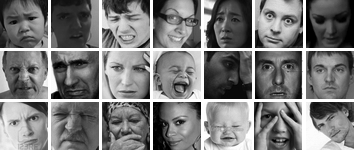
\includegraphics{Images/FER-2013.png}
    \caption{Imágenes extraídas de la base de datos FER-2013 \cite{Pramerdorfer}.}
    \label{fig:FER-2013}
\end{figure}

FER-2013 es la base de datos estáticos de expresiones faciales de mayor relevancia disponible públicamente. Consta de 35\,887 representaciones en escala de grises adquiridas de entornos no acondicionados expresamente con una resolución de $48 \times 48$ píxeles. Este conjunto reúne rostros de distinta naturaleza en términos de edad, orientación de la cara, etnia y género, tal y como puede observase en la \autoref{fig:FER-2013} y está dividido en tres subgrupos: entrenamiento, validación y evaluación con 28\,709, 3\,589 y 3\,589 muestras respectivamente. Asimismo, cada una de las imágenes está etiquetada con respecto a la expresión manifestada por el sujeto en la fotografía.

\begin{table}
\centering
\begin{tabular}{c|c|c|c|c|c|c|c|}
    \cline{2-8}
    & \textbf{Ira} & \textbf{Asco} & \textbf{Miedo} & \textbf{Alegría} & \textbf{Tristeza} & \textbf{Sorpresa} & \textbf{Neutral} \\ \hline
    \multicolumn{1}{|c|}{\textbf{\begin{tabular}[c]{@{}c@{}}Núm. de\\ imágenes\end{tabular}}} & 4\,953 & 547 & 5\,121 & 8\,989 & 6\,077 & 4\,002 & 6\,198 \\ \hline
\end{tabular}
\caption{Número de imágenes por cada expresión facial de la base de datos FER-2013.}
\label{Table:FER-2013}
\end{table}

En la \autoref{Table:FER-2013} se muestra la cantidad de imágenes en esta base de datos de las seis expresiones básicas y la expresión neutral. Como puede advertirse, hay un desequilibrio de clases notable, hecho que va a influir negativamente en el desempeño del modelo, especialmente para las emociones con menor representación. Como solución parcial a este problema se plantean en la \autoref{Chapter:DataAugmentation} una serie de técnicas de aumento de datos.

Por último, cabe destacar que la precisión humana sobre este conjunto es de aproximadamente $65\pm 5\%$ \cite{FER-2013_human_acc}.

\section{OpenCV} \label{Chapter:OpenCV}

OpenCV es una librería de código abierto de visión por computador escrita en C\slash C\texttt{++} y con un fuerte enfoque en aplicaciones en tiempo real. Por este motivo y teniendo en cuenta su extendido uso, es la que se va a utilizar para el desarrollo del software encargado de detectar y capturar el rostro de forma periódica y en pseudo tiempo real para la posterior identificación de la expresión facial o, dicho de otra forma, para la confección del espejo inteligente. Las características y la descripción detallada de los algoritmos empleados para tal fin se exponen en la \autoref{Chapter:FaceDetection}.

Por su parte, la implementación de este sistema se va a llevar a cabo mediante Python y, dado que OpenCV fue diseñada para ser efectiva computacionalmente, en un sistema operativo GNU/Linux optimizado para el hardware de la Raspberry PI.

    \chapter{Modelos Propuestos} \label{Chapter:4}
\section{Introducción}
%In order to enable a fair comparison with the results in Section II, we use the exact same dataset, preprocessing, as well as training and testing protocols.

\section{Afinación del Modelo Inception-v3}
\subsection{Preprocesamiento de los datos}
\subsection{Arquitectura}

%Additionally, this paper uses Average Pooling instead of Fully Connected layers at the topof the ConvNet, eliminating a large amount of parameters that do not seem to matter much.There are also several followup versions to the GoogLeNet, most recently Inception-v4.

\subsection{Entrenamiento}

\subsection{Resultados}




\section{Afinación del Modelo Inception-ResNet-v2}

\subsection{Preprocesamiento de los datos}

\subsection{Arquitectura}

\subsection{Entrenamiento}

\subsection{Resultados}



\section{Afinación del Modelo ResNet-50}

\subsection{Preprocesamiento de los datos}

\subsection{Arquitectura}

\subsection{Entrenamiento}

\subsection{Resultados}




\section{CycleGAN - Extensión de la Base de Datos FER-2013}

\subsection{Preprocesamiento de los datos}

\subsection{Arquitectura}

\subsection{Entrenamiento}

\subsection{Resultados}
    \renewcommand{\itemautorefname}{Punto}

\chapter{Modelos Propuestos} \label{Chapter:5}

Tal y como se ha comentado en la \autoref{Chapter:TransferLearning}, la explotación de las técnicas de transferencia de aprendizaje y por lo tanto el empleo de unos modelos con una serie de pesos ya definidos con respecto a un conjunto de datos determinado, constituyen la base de los sistemas propuestos en este capítulo.

\begin{figure}
    \centering
    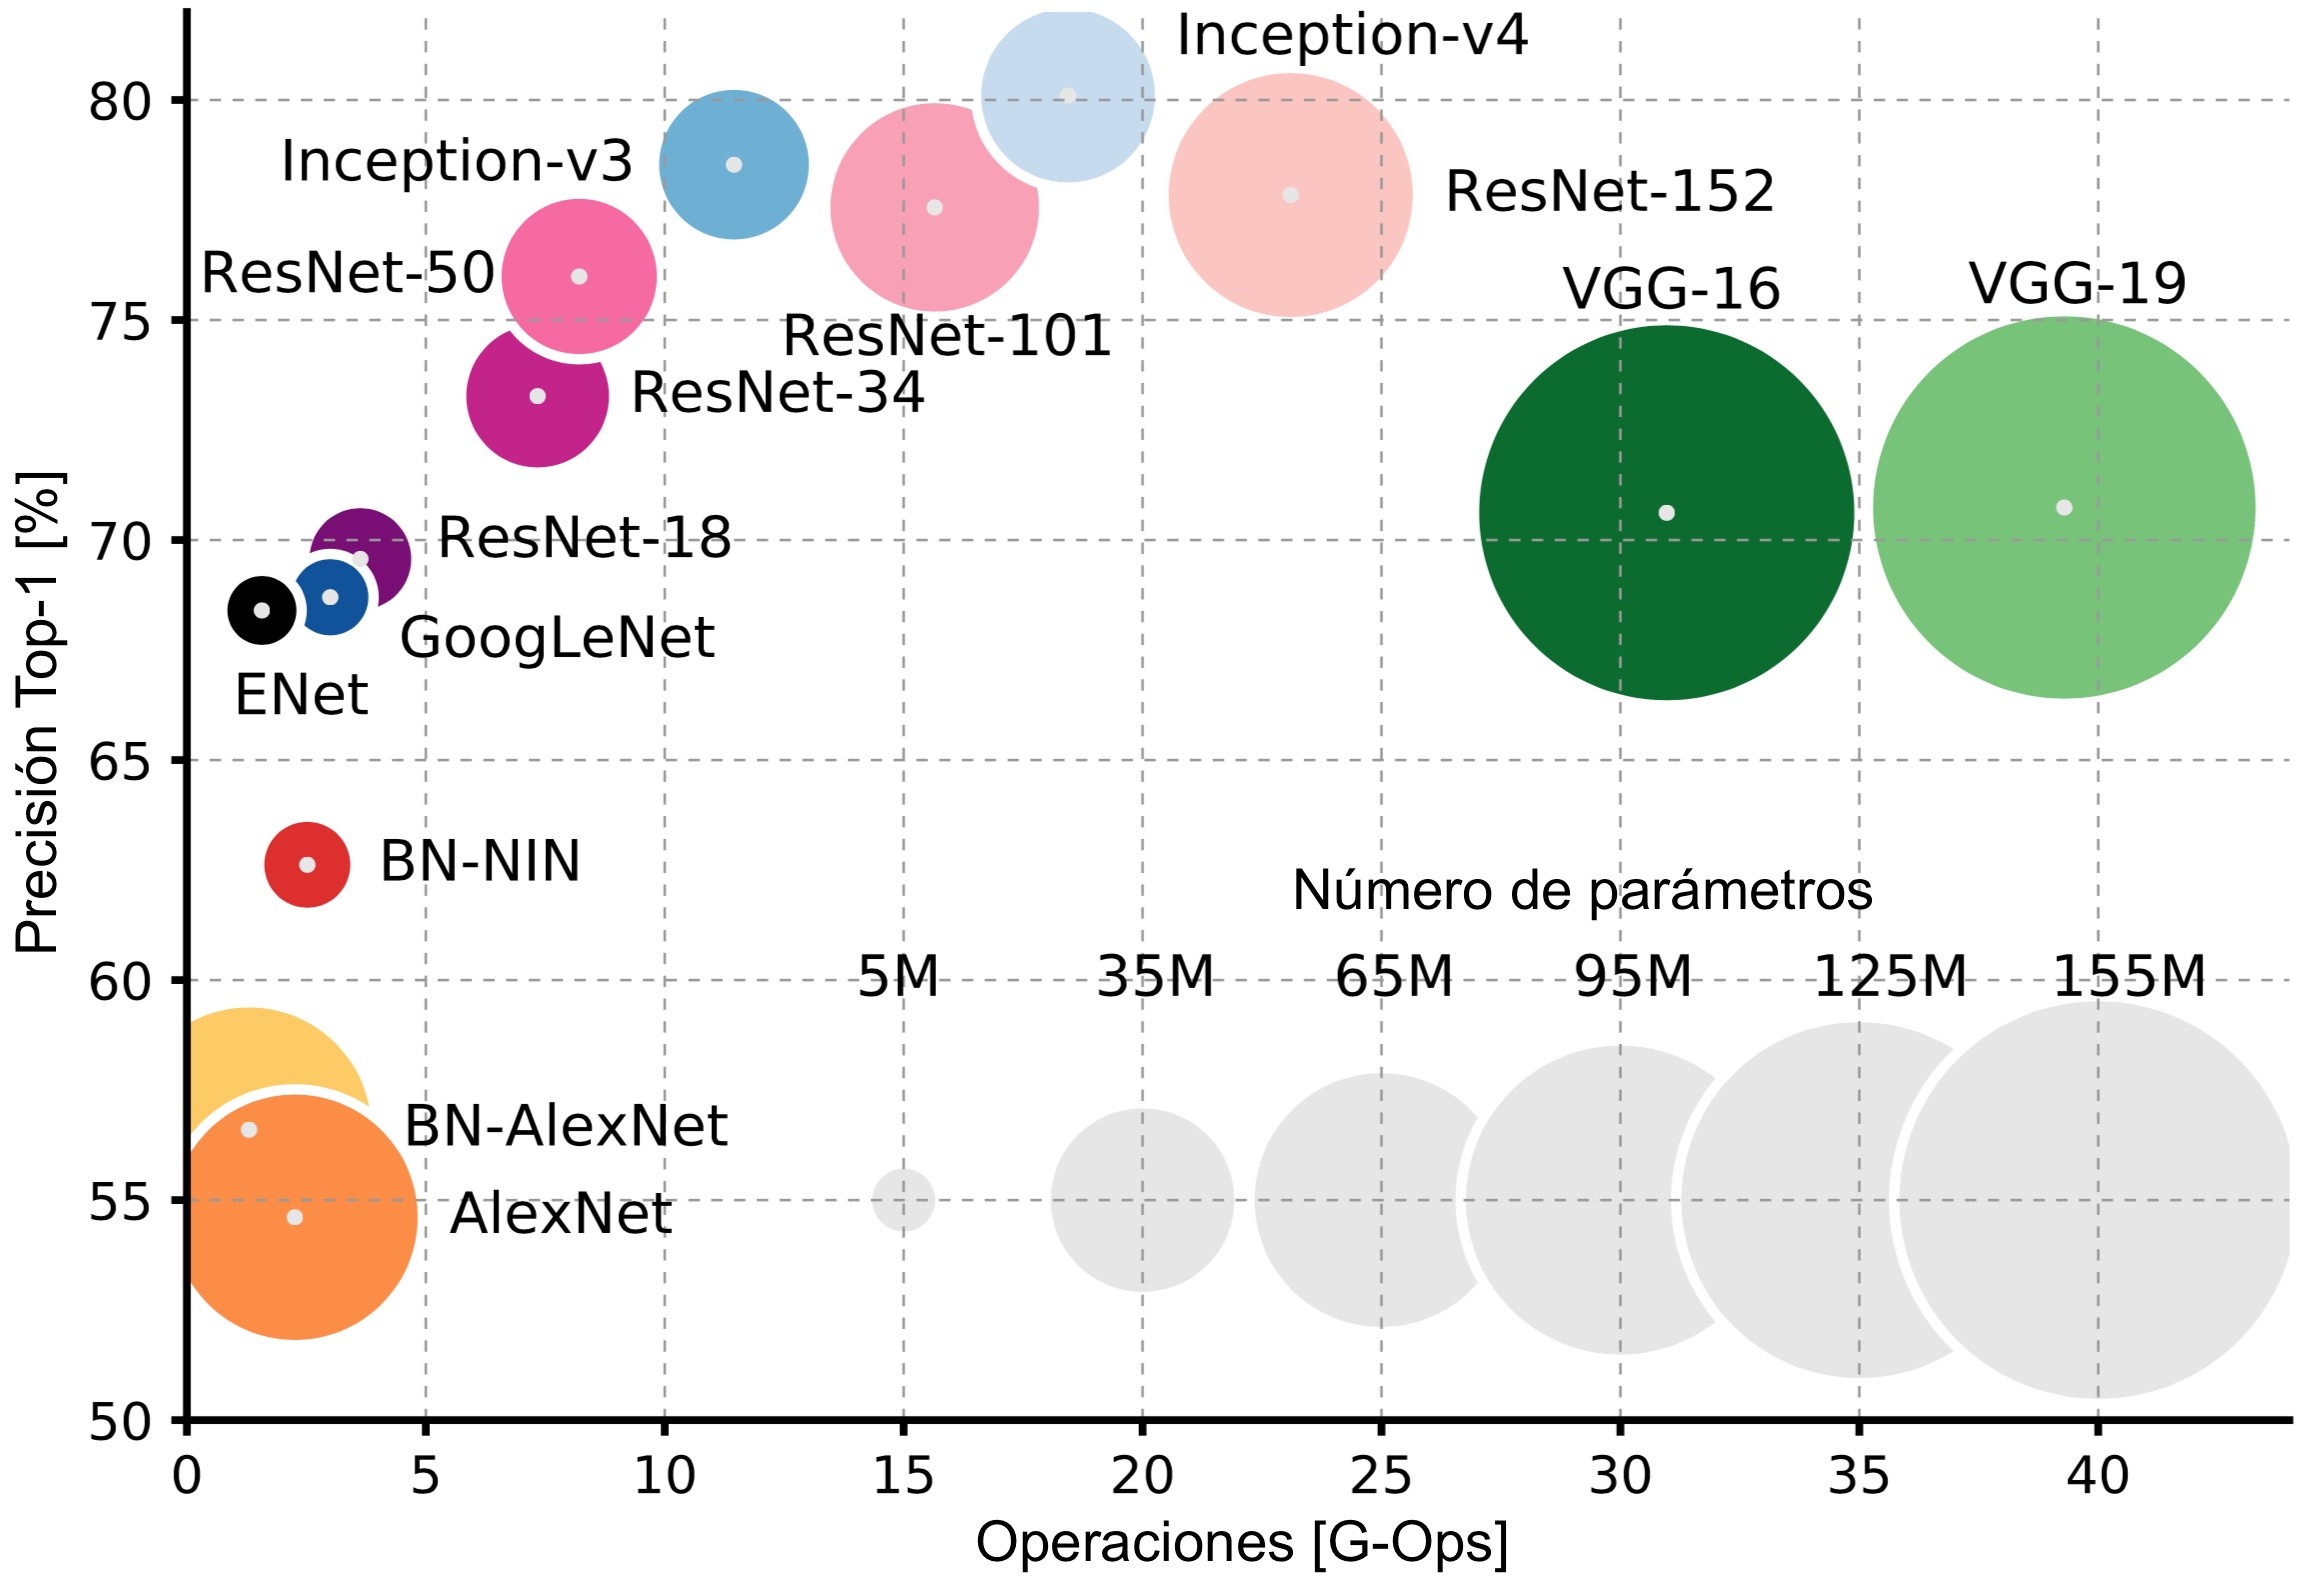
\includegraphics[scale=0.25]{Images/Models.png}
    \caption{Precisión Top-1 frente al coste computacional de una iteración del proceso de aprendizaje y el número de parámetros de la red \cite{Models}. Cabe destacar que aunque el modelo Inception-ResNet-v2 no se incluya en la figura, presenta características muy similares a Inception-v4 \cite{Inception-ResNet}.}
    \label{fig:Models}
\end{figure}

Por consiguiente, son utilizados en primera instancia los modelos Inception-v3 \cite{Inception-v3} e Inception-ResNet-v2 \cite{Inception-ResNet} con los pesos entrenados previamente sobre el conjunto de datos ImageNet descrito en la \autoref{Chapter:ImageNet}. Sin embargo, dado que las propiedades de las imágenes de esta base de datos difieren en gran medida de las características faciales que se intentan aprender y reconocer, se ha optado por explorar el uso de modelos más sencillos pero enfocados al reconocimiento facial. Es por ello que en última instancia se emplea el modelo ResNet-50 preetrenado con la base de datos VGGFace2 expuesta en la \autoref{Chapter:VGGFace2}. La comparación de estos modelos en el desempeño del desafío ILSVRC puede observarse en la \autoref{fig:Models}. Esta representación, además, escenifica la principal razón de la elección de estos modelos concretos: son los que mejores tasas obtienen con respecto al coste computacional y al número de parámetros.

Por último, obtenidos unos resultados más que aceptables y eficientes en lo que respecta al tiempo de entrenamiento, se ha intentado dar un paso más allá con la intención de mejorar las tasas de acierto y la calidad de la base de datos inicial mediante la implementación de una Red Generativa Antagónica (GAN) que permita la producción artificial de imágenes y, por lo tanto, la eliminación del desequilibrio de la distribución de clases del conjunto FER-2013.

En definitiva, a lo largo del proceso de desarrollo de un sistema de reconocimiento de expresiones faciales válido, se han ido explorando numerosas arquitecturas (Inception-v3, Inception-ResNet-v2 y ResNet-50) y técnicas (aumento de datos) con el objetivo de ir obteniendo cada vez mejores resultados sobre la base de datos FER-2013. Asimismo, a fin de permitir una comparación justa con respecto a los resultados de la \autoref{Chapter:RelatedWork}, son utilizados los protocolos de uso estipulados inicialmente por este desafío y que establecen la división de esta base de datos en tres conjuntos diferentes: entrenamiento, validación y evaluación.

\section{Afinación del Modelo Inception-v3}

Inception-v3 ha sido el resultado de las investigaciones llevadas a cabo por el equipo de Google para conseguir un modelo con una arquitectura cada vez más profunda e inteligente y capaz de desenvolverse de forma eficiente, tanto computacionalmente como cualitativamente, en el desafío ILSVR.

%Su diseño, motivado por los experimentos a gran escala llevados a cabo sobre distintas redes convolucionales, gira en torno a cuatro principios %básicos \cite{Inception-v3}:
%\begin{enumerate}
%  \item Evitar los cuellos de botella, de modo que los datos fluyan de forma uniforme a lo largo de la red.
%  \item Aumentar el número de dimensiones a medida que la información avance por la red. Las redes, de esta forma, se entrenarán más rápido.
%  \item Bajar la resolución de la entrada antes de una capa convolucional promueve un aprendizaje más rápido y no da lugar a pérdidas %significativas de la ganancia de información.
%  \item Equilibrar el ancho y la profundidad de la red aumenta el rendimiento de las redes neuronales. \label{item:4}
%\end{enumerate}

\subsection{Arquitectura}

\begin{figure}
    \centering
    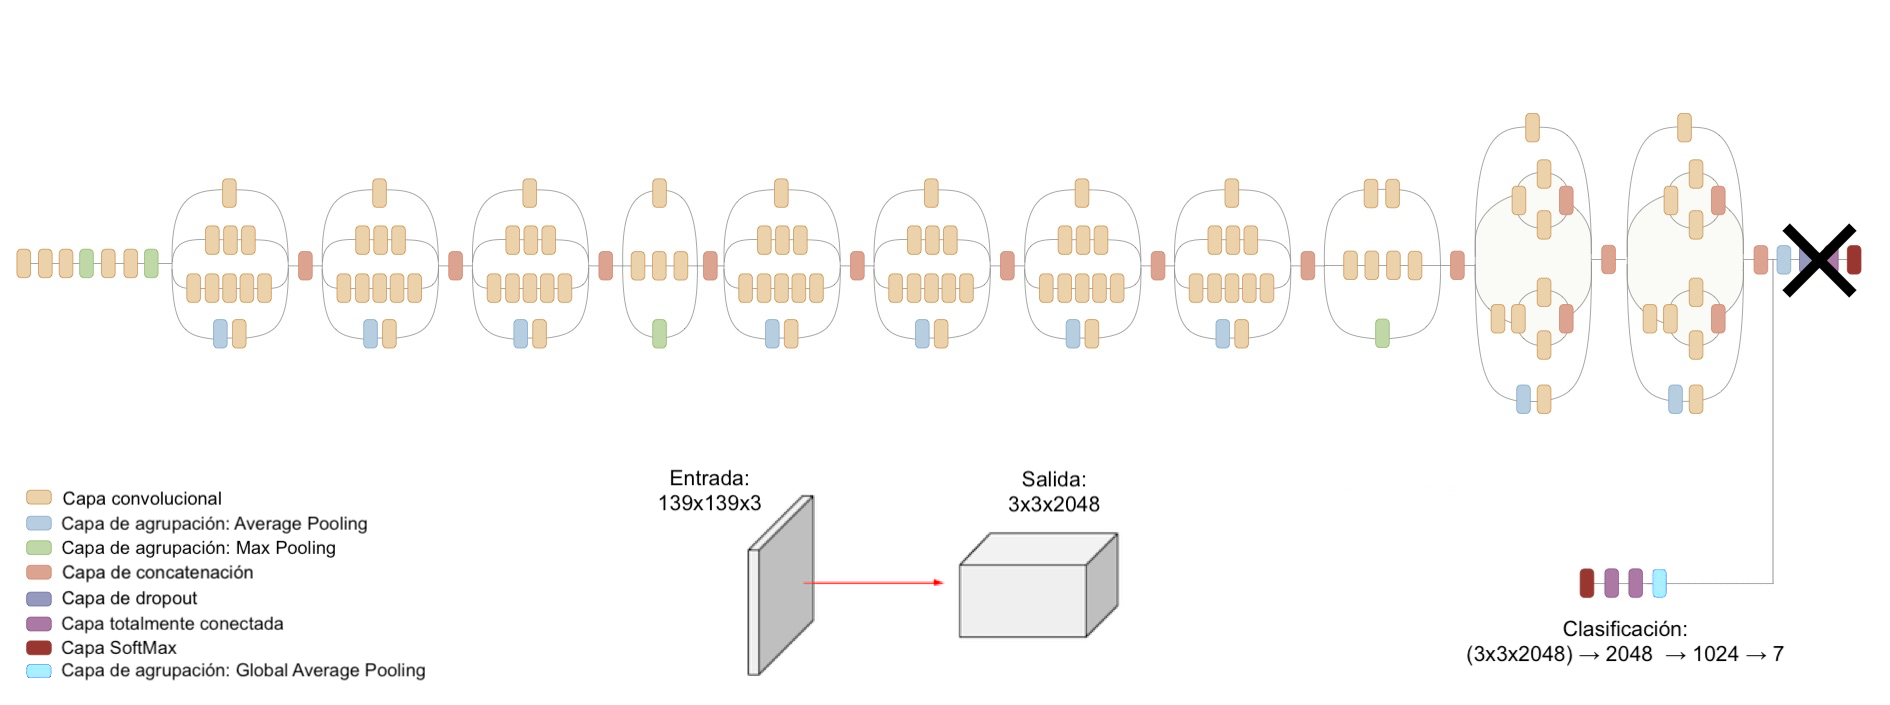
\includegraphics[width=\textwidth]{Images/Inception-v3.png}
    \caption{Arquitectura del modelo Inception-v3 adaptado al problema del reconocimiento de expresiones faciales \cite{img:Inception-v3}.}
    \label{fig:Inception-v3}
\end{figure}

\begin{figure}
    \centering
    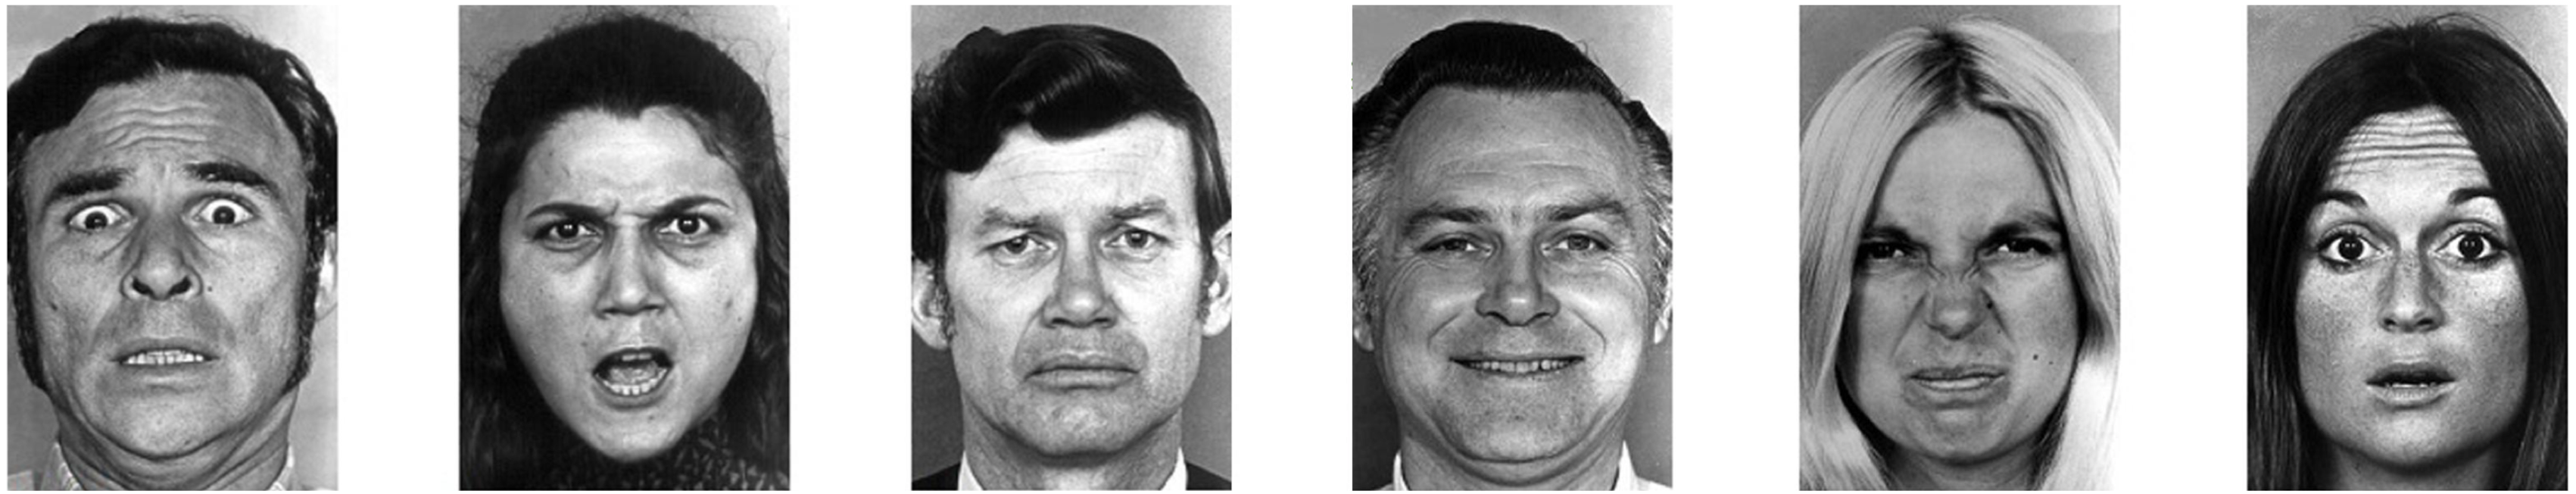
\includegraphics[width=\textwidth]{Images/emotions.png}
    \caption{\cite{Inception-v3}.}
    \label{fig:InceptionModule}
\end{figure}

En la \autoref{fig:Inception-v3} se muestra la estructura simplificada y adaptada al problema del reconocimiento de expresiones faciales del modelo Inception-v3. Esta arquitectura propuesta es básicamente una sucesión de tramos convolucionales y no linealidades, empleándose la función de activación ReLU y la normalización por lotes en cada una de las etapas, aunque esto último no se muestre explícitamente en la representación anteriormente mencionada. Como se ha podido advertir, la característica principal de este modelo es el hecho de que el flujo de datos a lo largo de algunas secciones de esta red no es secuencial, sino que se realiza en paralelo. Estas agrupaciones son conocidas como módulos Inception y representan la solución a los problemas de eficiencia de las redes estado del arte predecesoras, cumpliendo, además, la misma función y obteniendo los mismos resultados que una capa convolucional estándar. Las diferentes estructuras de estos módulos empleados por el modelo Inception-v3 pueden observarse en la \autoref{fig:InceptionModules}. La idea detrás de estas disposiciones paralelas es que dada la misma entrada para varias capas convolucionales o de agrupación de distinto tamaño se generen características únicas para cada una de ellas que posteriormente procederán a concatenarse. Este enfoque, sin embargo, da lugar a una salida con una profundidad extremadamente grande que es solucionada principalmente mediante la utilización de filtros convolucionales $1\times 1$, especialmente efectivos para reducir la dimensionalidad \cite{NetworkInNetwork}, justo antes de las capas convolucionales de mayor tamaño. Otro de los puntos que es explotado por los módulos Inception es la sustitución de los filtros tradicionales de tamaño $n\times n$ por una secuencia de capas convolucionales de dimensionest $1\times n$ y $n \times 1$. Mediante esta técnica se consigue disminuir drásticamente los costes computacionales a medida que $n$ aumenta. En la práctica y tal como se ha visto en la \autoref{fig:InceptionModules}, son utilizados básicamente filtros con $n = 7$ y $n = 3$.

Por otro lado, dado que esta red ha sido diseñada para el reto de ImageNet, ha sido necesario sustituir la etapa de clasificación del modelo Inception-v3 original, tal y como se ha visto en la \autoref{fig:Inception-v3}. De esta forma, en primer lugar se ha introducido una capa basada en la agrupación promedio global, que impone la correspondencia entre los mapas de activación y las clases, reduce el número de parámetros y además es menos propensa al sobreaprendizaje que las capas convencionales totalmente conectadas \cite{NetworkInNetwork}. Posteriormente y con la finalidad de reducir la dimensionalidad de la red de una manera suave a las 7 clases correspondientes a las expresiones faciales que se pretenden clasificar, se han insertado dos capas totalmente conectadas.

\subsection{Preprocesamiento de los datos de entrenamiento}


\subsection{Entrenamiento}

\subsection{Resultados}



\cite{Inception-v3}




\section{Afinación del Modelo Inception-ResNet-v2}

\cite{Inception-ResNet}

\subsection{Preprocesamiento de los datos}

\subsection{Arquitectura}

\subsection{Entrenamiento}

\subsection{Resultados}








\section{Afinación del Modelo ResNet-50}
\cite{ResNet}

\subsection{Preprocesamiento de los datos}

\subsection{Arquitectura}

\subsection{Entrenamiento}

\subsection{Resultados}




\section{CycleGAN - Extensión de la Base de Datos FER-2013}

\subsection{Preprocesamiento de los datos}

\subsection{Arquitectura}

\subsection{Entrenamiento}

\subsection{Resultados}
    \chapter{Extensión de la Base de Datos FER-2013 } \label{Chapter:6}

Obtenidos unos resultados más que aceptables y eficientes en lo que respecta al tiempo de entrenamiento, se ha intentado dar un paso más allá con la intención de mejorar las tasas de acierto y la calidad de la base de datos inicial mediante la implementación de una Red Generativa Antagónica de Ciclo Consecuente (CycleGAN) \cite{cycleGAN} que permita la producción artificial de imágenes y, por lo tanto, la eliminación del desequilibrio de la distribución de clases del conjunto FER-2013. En un principio tan sólo se pretende aumentar el número de datos etiquetados con la expresión facial de asco, que como se vio en la \autoref{Table:FER-2013} es con diferencia el gesto con menor representación. Las imágenes a partir de las cuales se pretenderá generar esta última emoción corresponderán, dada la adaptabilidad de su naturaleza, a la clase de la expresión neutral.

\section{Arquitectura propuesta}

\begin{figure}
    \centering
    \begin{subfigure}[t]{0.8\textwidth}
      \centering
      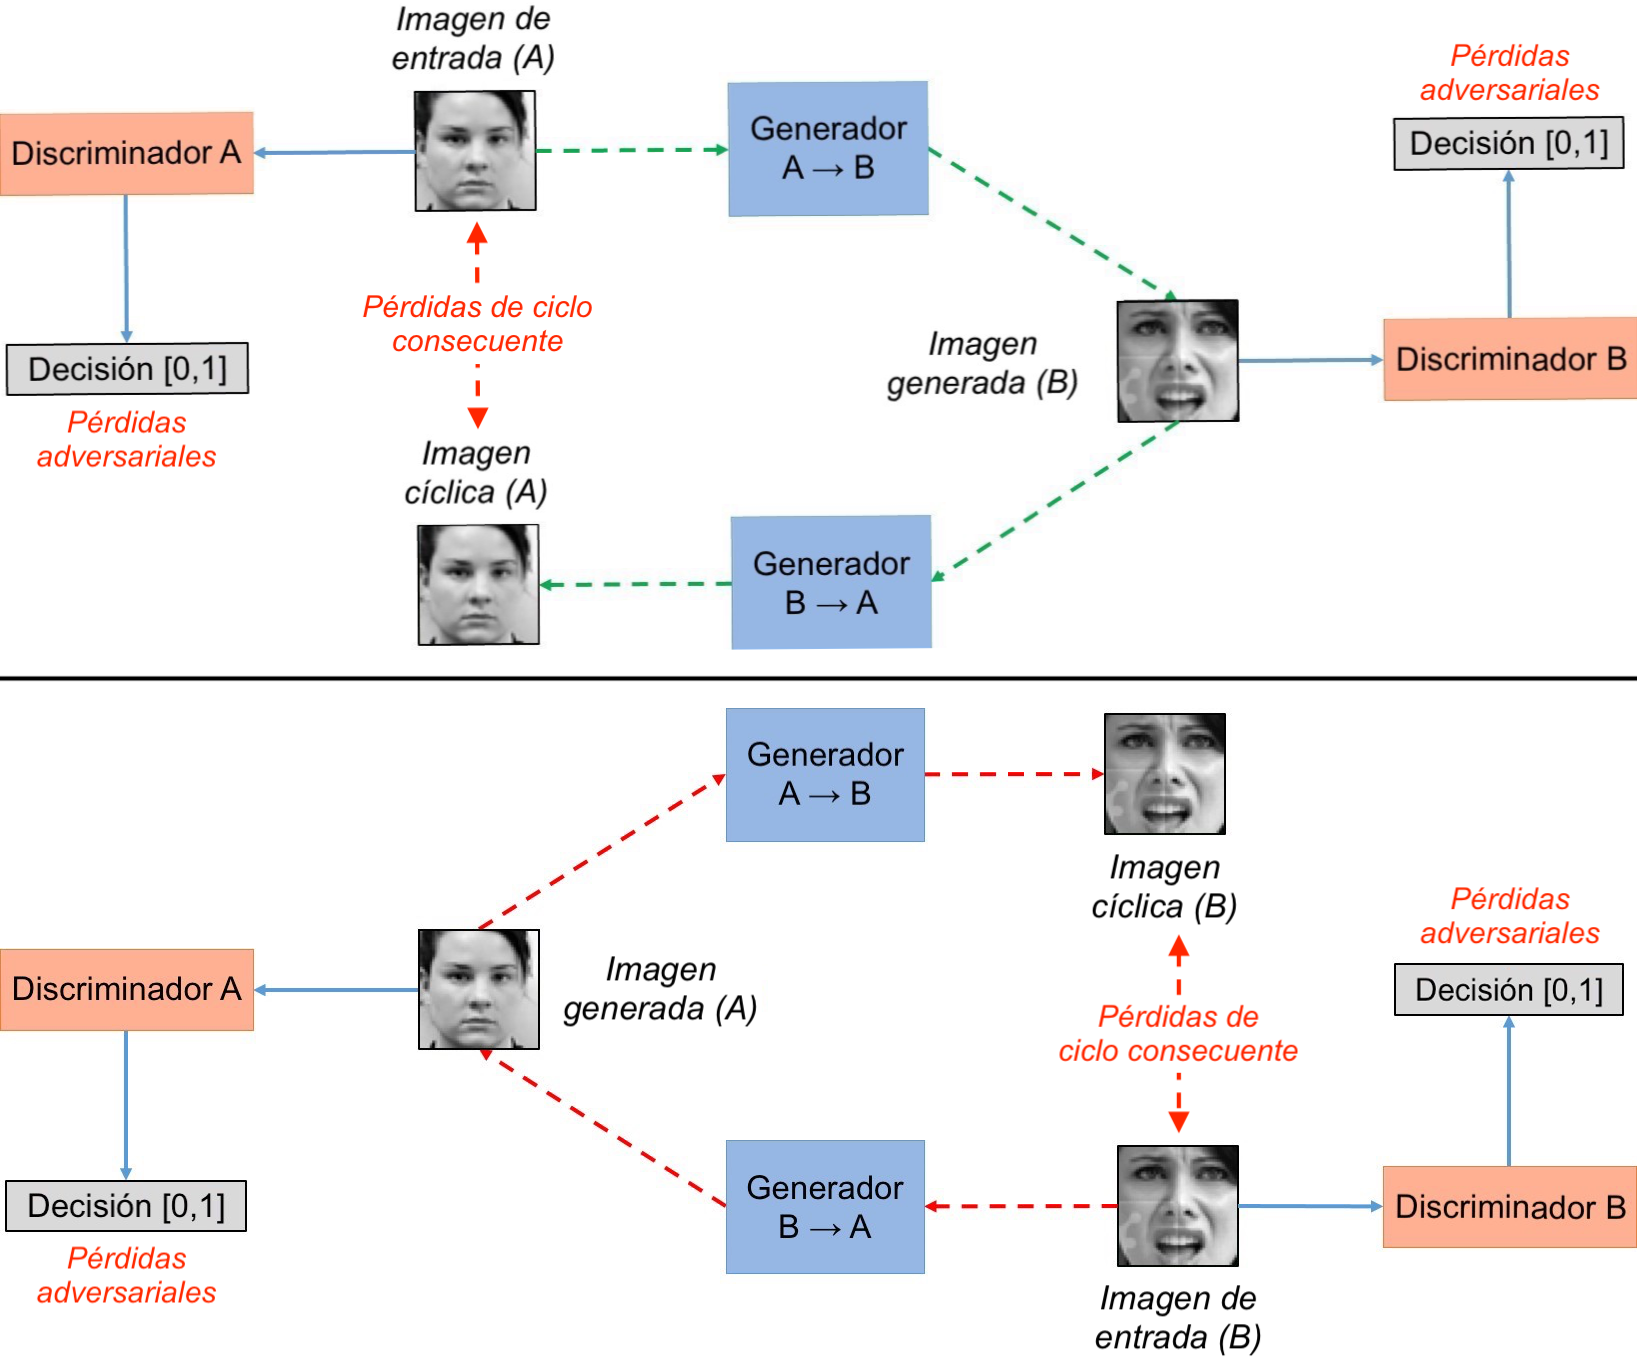
\includegraphics[width=\linewidth]{Images/CycleGANArchitecture.png}
      \caption{Estructura completa de la red CycleGAN.}
      \label{fig:CycleGAN_general}
    \end{subfigure}
    
    \vspace{1cm}
    \begin{subfigure}[t]{0.8\textwidth}
      \centering
      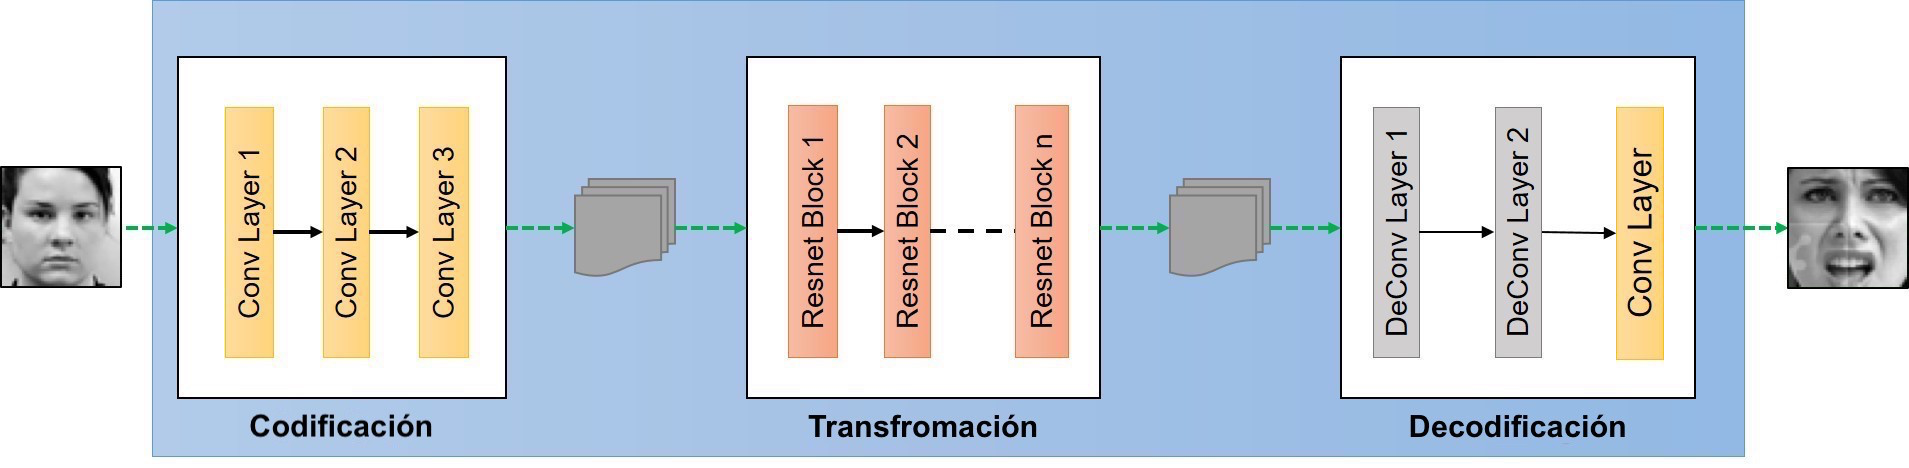
\includegraphics[width=\linewidth]{Images/Generator.png}
      \caption{Arquitectura simplificada del generador de la red CycleGAN.}
      \label{fig:Generator}
    \end{subfigure}
    
    \vspace{1cm}
    \begin{subfigure}[t]{.7\textwidth}
      \centering
      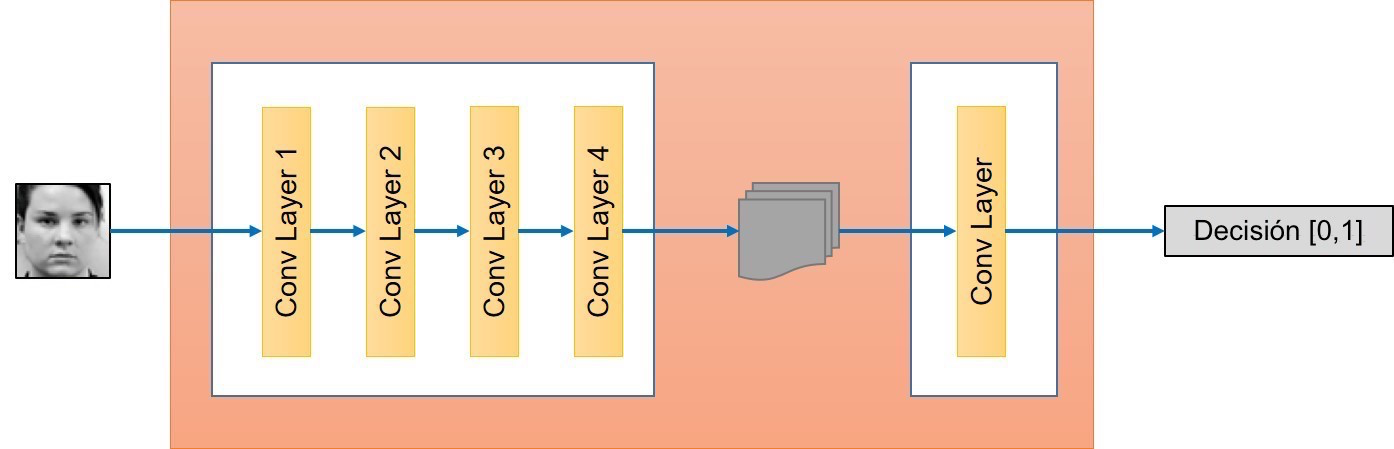
\includegraphics[width=\linewidth]{Images/Discriminator.png}
      \caption{Arquitectura simplificada del discriminador de la red CycleGAN.}
      \label{fig:Discriminator}
    \end{subfigure}
    \caption{Arquitectura esquematizada y simplificada de la Red Generativa Antagónica de Ciclo Consecuente \cite{img:CycleGAN}.}
    \label{fig:CycleGANArchitecture}
\end{figure}

La arquitectura aquí desarrollada y esquematizada en la \autoref{fig:CycleGANArchitecture} es una adaptación de la estructura propuesta en el documento original de las redes CycleGAN y que ha demostrado unos resultados más que razonables en el área de las redes generativas de base neuronal. Asimismo, al igual que los modelos descritos anteriormente, el acondicionamiento se ha llevada a cabo íntegramente en la API de Keras y sobre TensorFlow.

\subsection{Red generadora}

Desde un enfoque de alto nivel es posible dividir la red del generador en 3 módulos distintos dispuestos según la \autoref{fig:Generator}:
\begin{itemize}
    \item \textbf{Módulo de codificación}. Está formado por 3 capas convolucionales que extraen las características superficiales y disminuyen el mapa de activación de la imagen inyectada.
    \item \textbf{Módulo de transformación}. Dado que el objetivo de los procesos de aumento de datos es la retención de ciertas características de la entrada original, como el tamaño y la forma del rostro en este caso, se hace evidente que para este tipo de transformaciones puede resultar especialmente efectivo utilizar arquitecturas residuales, que además favorecen la estabilización de las respuestas de las redes profundas. Es por todo ello que en el contexto particular y en el documento original son empleados básicamente 6 módulos residuales (\autoref{fig:ResNetBlock}) constituidos por filtros convolucionales de tamaño reducido ($3\times 3$).
    \item \textbf{Módulo de decodificación}. Su función es exactamente la opuesta al primer módulo ya que es precisamente el que trata de reconstruir y trasladar la imagen original etiquetada con la emoción neutral al dominio objetivo que corresponde a la expresión de asco. Para tal fin se emplean dos capas deconvolucionales que recomponen el ancho y el alto de la imagen y una última capa convolucional que restaura los canales RGB de la representación inicial.
\end{itemize}

Asimismo, cabe destacar que son utilizadas en cada una de las capas la función de activación ReLU con fugas y la normalización de instancias. Esta última es una sustitución de la técnica de normalización por lotes y es empleada en este proyecto por las mejoras drásticas y demostrables que permite obtener a las redes neuronales profundas en las tareas de generación de datos \cite{InstanceNormalization}. Intuitivamente, este tipo de normalización consigue que la distribución de cada una de las imágenes de un determinado lote parezca gaussiana, lo que permite eliminar información específica y por lo tanto simplificar y optimizar la generación.

En cuanto a la ReLU con fugas, ésta ha reportado mejores resultados en las redes generativas que la ReLU tradicional ya que parece cubrir el espacio de color de una forma más optimizada \cite{GAN}. Igualmente, esta función de activación es el intento de resolver el problema de la muerta de las ReLU convencionales, que para valores menores que cero desactivan la neurona, y por lo tanto del desvanecimiento del gradiente en esas unidades que paralizan el aprendizaje. Su expresión matemática se expone en la \autoref{eq:LeakyReLU}.
\begin{align} \label{eq:LeakyReLU}
    f(x) &= max(x, \alpha x) &\forall \alpha \leq 1 \\
    \text{donde}~ 
    \alpha &\equiv \text{constante} \notag
\end{align}
En el documento original y en el caso particular de este proyecto se toma $\alpha = 0.2$.

\subsection{Red discriminativa}

La función de esta red es básicamente tratar de predecir si la imagen introducida en su entrada es real o procede de la salida del generador. En este caso su arquitectura, representada en la \autoref{fig:Discriminator}, presenta una estructura simple de 5 capas convolucionales de tamaño $4\times 4$ apiladas con una mínima alteración en el último nivel para permitir el cálculo del error de mínimos cuadrados del discriminador \cite{LSGAN}, necesario para realizar la actualización periódica de la función de pérdidas según lo especificado en la \autoref{eq:GAN}. Esta ligera modificación consiste en la supresión de la función de activación y de la unidad de normalización de instancias.

\section{Entrenamiento}

\subsection{Preprocesamiento de los datos}

Teniendo en cuenta la diversidad de las imágenes del conjunto FER-2013, en esta ocasión tan solo se va a proceder a realizar un preprocesamiento sutil, que además permitirá disminuir el coste computacional de la red. Por ello, se realizan únicamente las siguientes transformaciones:
\begin{itemize}
    \item \textbf{Redimensionamiento}. Dado que la entrada de la arquitectura CycleGAN ha sido ajustada para aceptar las imágenes de la base de datos FER-2013 con la resolución por defecto ($48 \times 48$), tan solo se realiza una replicación de los datos en escala de gris a los tres espacios de color RGB.
    \item \textbf{Normalización}. El modelo de color RGB de las imágenes de la entrada se adapta al intervalo $[-1, 1]$ mediante la \autoref{eq:PreprocessInception} ya vista anteriormente.
    \item \textbf{Volteo horizontal}. Esta transformación geométrica de carácter aleatorio es la única que se va a aplicar en vista de su eficacia computacional y de enriquecimiento del conjunto de entrada.
\end{itemize}

\subsection{Proceso de Aprendizaje}

El proceso de entrenamiento de esta arquitectura ha seguido los puntos descritos en la \autoref{Chapter:CycleGan} y ha tenido como objetivo la reducción de las funciones de pérdidas detalladas en la \autoref{eq:CycleGAN} y mostradas gráficamente en la \autoref{fig:CycleGAN_general}. Asimismo, cabe destacar que los parámetros de este modelo han sido escogidos con respecto al artículo original que describe este tipo de redes generativas \cite{cycleGAN}:
\begin{itemize}
    \item \textbf{Inicialización}. En primer lugar y dado que esta red ha sido entrenada desde cero se ha visto necesario realizar una inicialización de los pesos a partir de una distribución gaussiana con una media de $0$ y una desviación estándar de $0.02$. 
    \item \textbf{Tamaño de los lotes}. Las imágenes se han alimentado en la red de una en una, lo que ha implicado también actualizar las funciones de pérdidas y los pesos en cada pasada.
    \item \textbf{Optimizador}. Se ha empleado el optimizador Adam con una tasa de aprendizaje de $ \lambda = 0.0002$ (\autoref{eq:Adam}), $\beta_1 = 0.5$ (\autoref{eq:AdamBeta1}) y $\beta_2 = 0.999$ (\autoref{eq:AdamBeta2}).
    \item \textbf{Peso de la función de pérdidas de ciclo consecuente}. Se le ha otrogado un valor de $\lambda = 10$ (\autoref{eq:CycleGAN}).
    \item \textbf{Iteraciones}. La red ha sido entrenada durante $7\,300$ iteraciones sobre los datos categorizados con las expresiones faciales de asco y neutral.
\end{itemize}

\subsection{Despliegue en la Plataforma Google Cloud}

En esta ocasión el entrenamiento en la plataforma de Google Cloud se ha realizado mediante la herramienta Cloud Machine Learning Engine descrita en la \autoref{Chapter:GoogleCloud} y empleando la GPU NVIDIA Tesla K80. Esto es debido a que ya no se presentan las limitaciones de memoria anteriormente existentes al utilizarse esta vez un número bastante inferior de imágenes que reúnen solo las emociones de la clases neutral y asco.

\section{Resultados}

En un primer momento y dado que en cada iteración el número de datos inyectados al modelo está limitado por la cantidad de imágenes de la clase con menor representación, en este caso la etiquetada con la expresión de asco, se estipuló un entrenamiento de $30\,000$ iteraciones considerando, además, los entornos comunes de implementación \cite{RSGAN}. Sin embargo y como se puede intuir, estos modelos son muy costosos de entrenar y más en situaciones como la aquí propuesta donde se intenta establecer una correlación entre una categoría con $4\,965$ imágenes (neural) y una con $436$ (asco). Por ello, debido a las limitaciones económicas de la prueba gratuita de Google Cloud, esta red únicamente ha podido ser entrenada durante $7\,300$ iteraciones, empleando para ello unas 57 horas aproximadamente.

En la \autoref{fig:CycleGAN_metrics} del \autoref{Appendix:Figures} se pueden consultar las pérdidas del generador y del discriminador de este entrenamiento parcial. Desafortunadamente, éstas son muy poco intuitivas ya que la mejora de las métricas de uno de estos dos módulos implica la degradación de la respuesta del otro. El funcionamiento esperado, por lo tanto, es que tanto las pérdidas del generador como las del discriminador converjan hacia valores constantes.

\begin{figure}
    \centering
    \begin{subfigure}[t]{.45\textwidth}
      \centering
      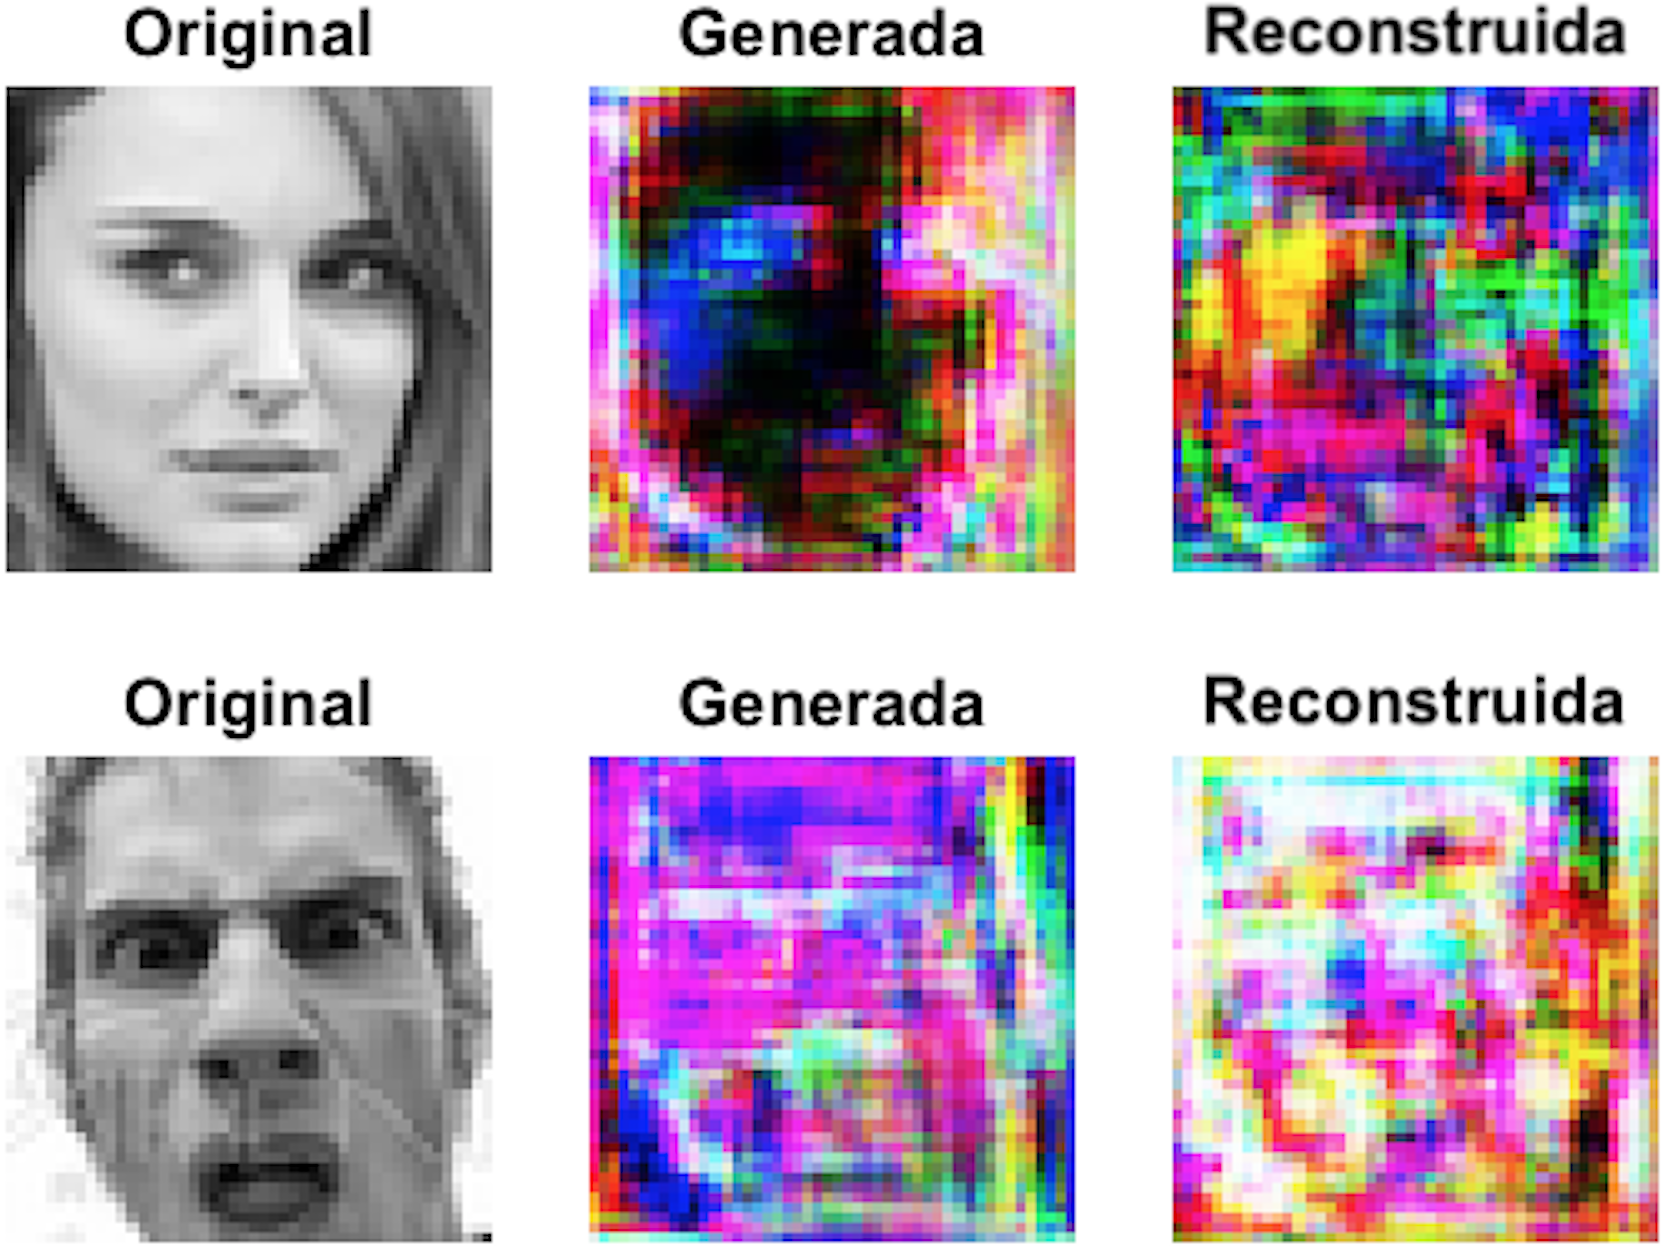
\includegraphics[width=\linewidth]{Images/CycleGAN_0.png}
      \caption{Imágenes extraídas en la iteración $0$.}
      \label{fig:CycleGAN_0}
    \end{subfigure}
    \hfill
    \begin{subfigure}[t]{.45\textwidth}
      \centering
      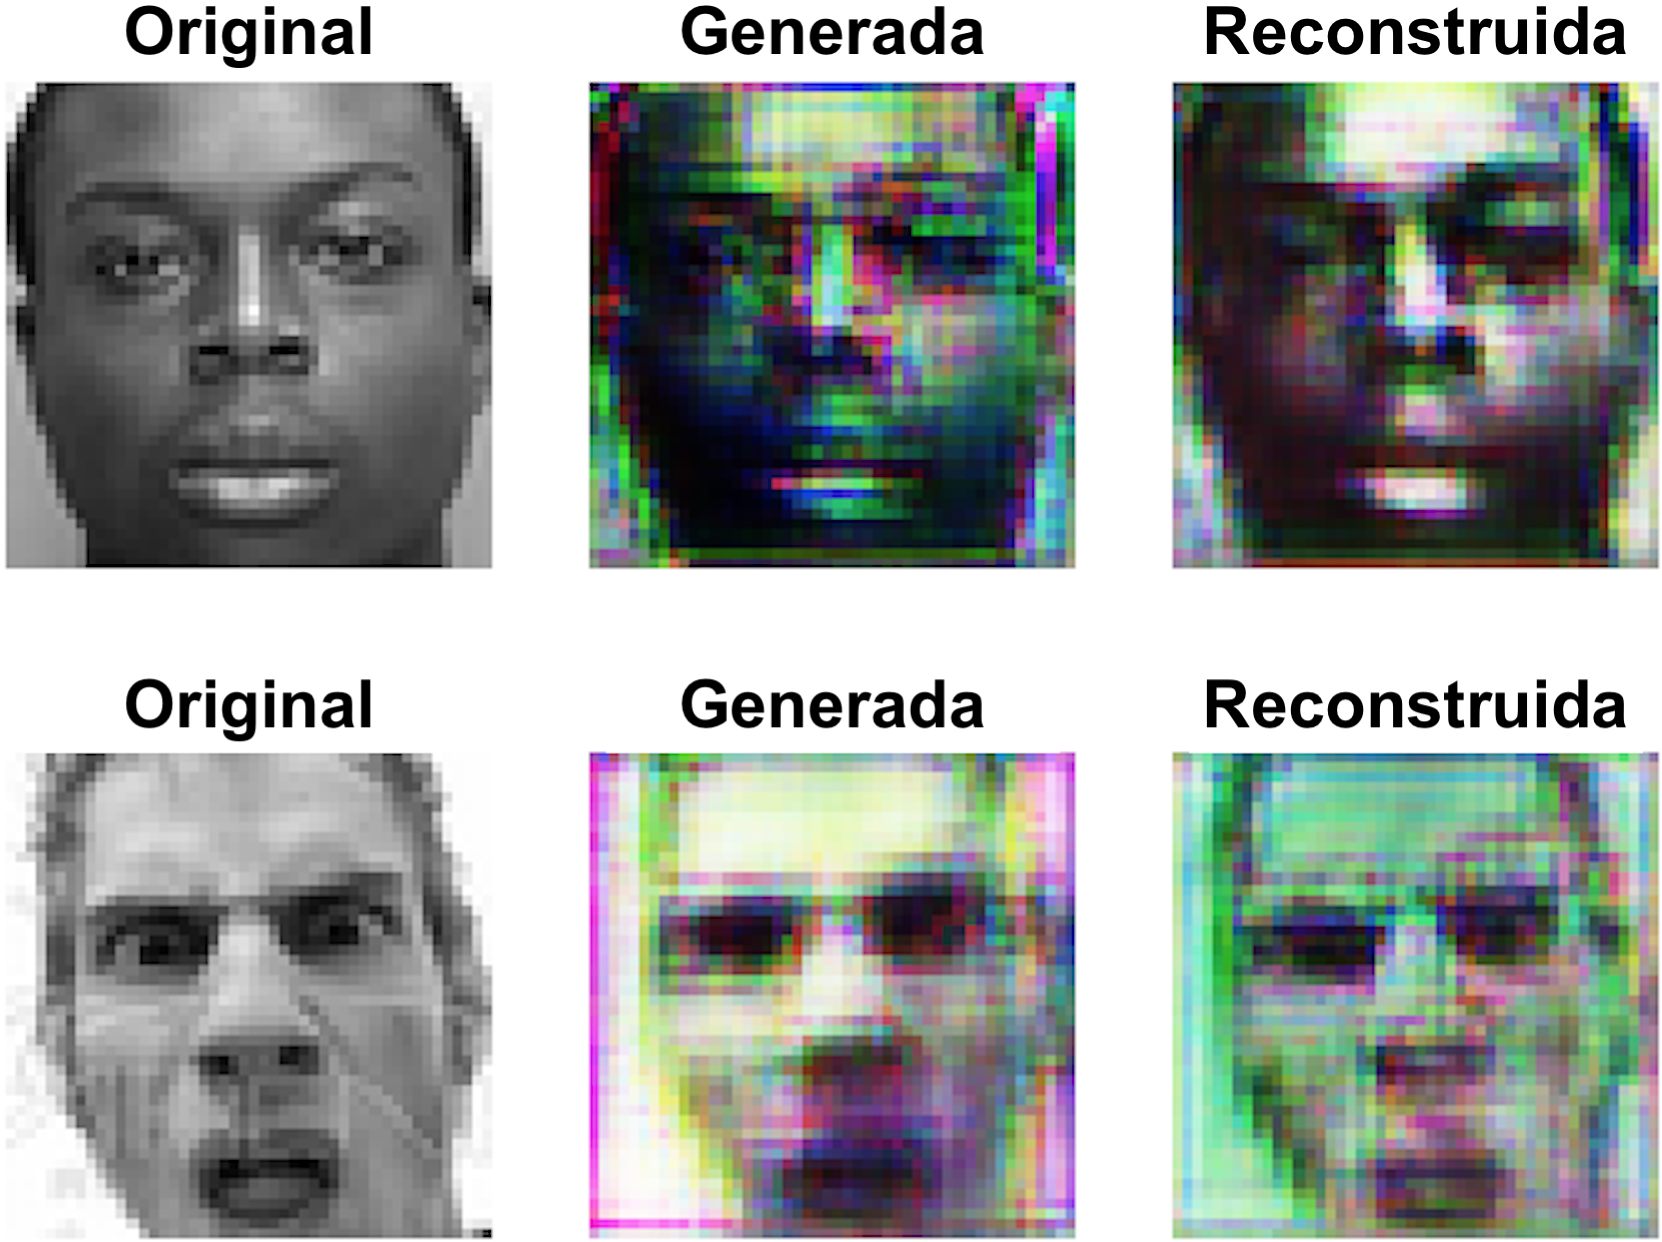
\includegraphics[width=\linewidth]{Images/CycleGAN_500.png}
      \caption{Imágenes extraídas en la iteración $500$.}
      \label{fig:CycleGAN_500}
    \end{subfigure}
    
    \vspace{1cm}
    \begin{subfigure}[t]{.45\textwidth}
      \centering
      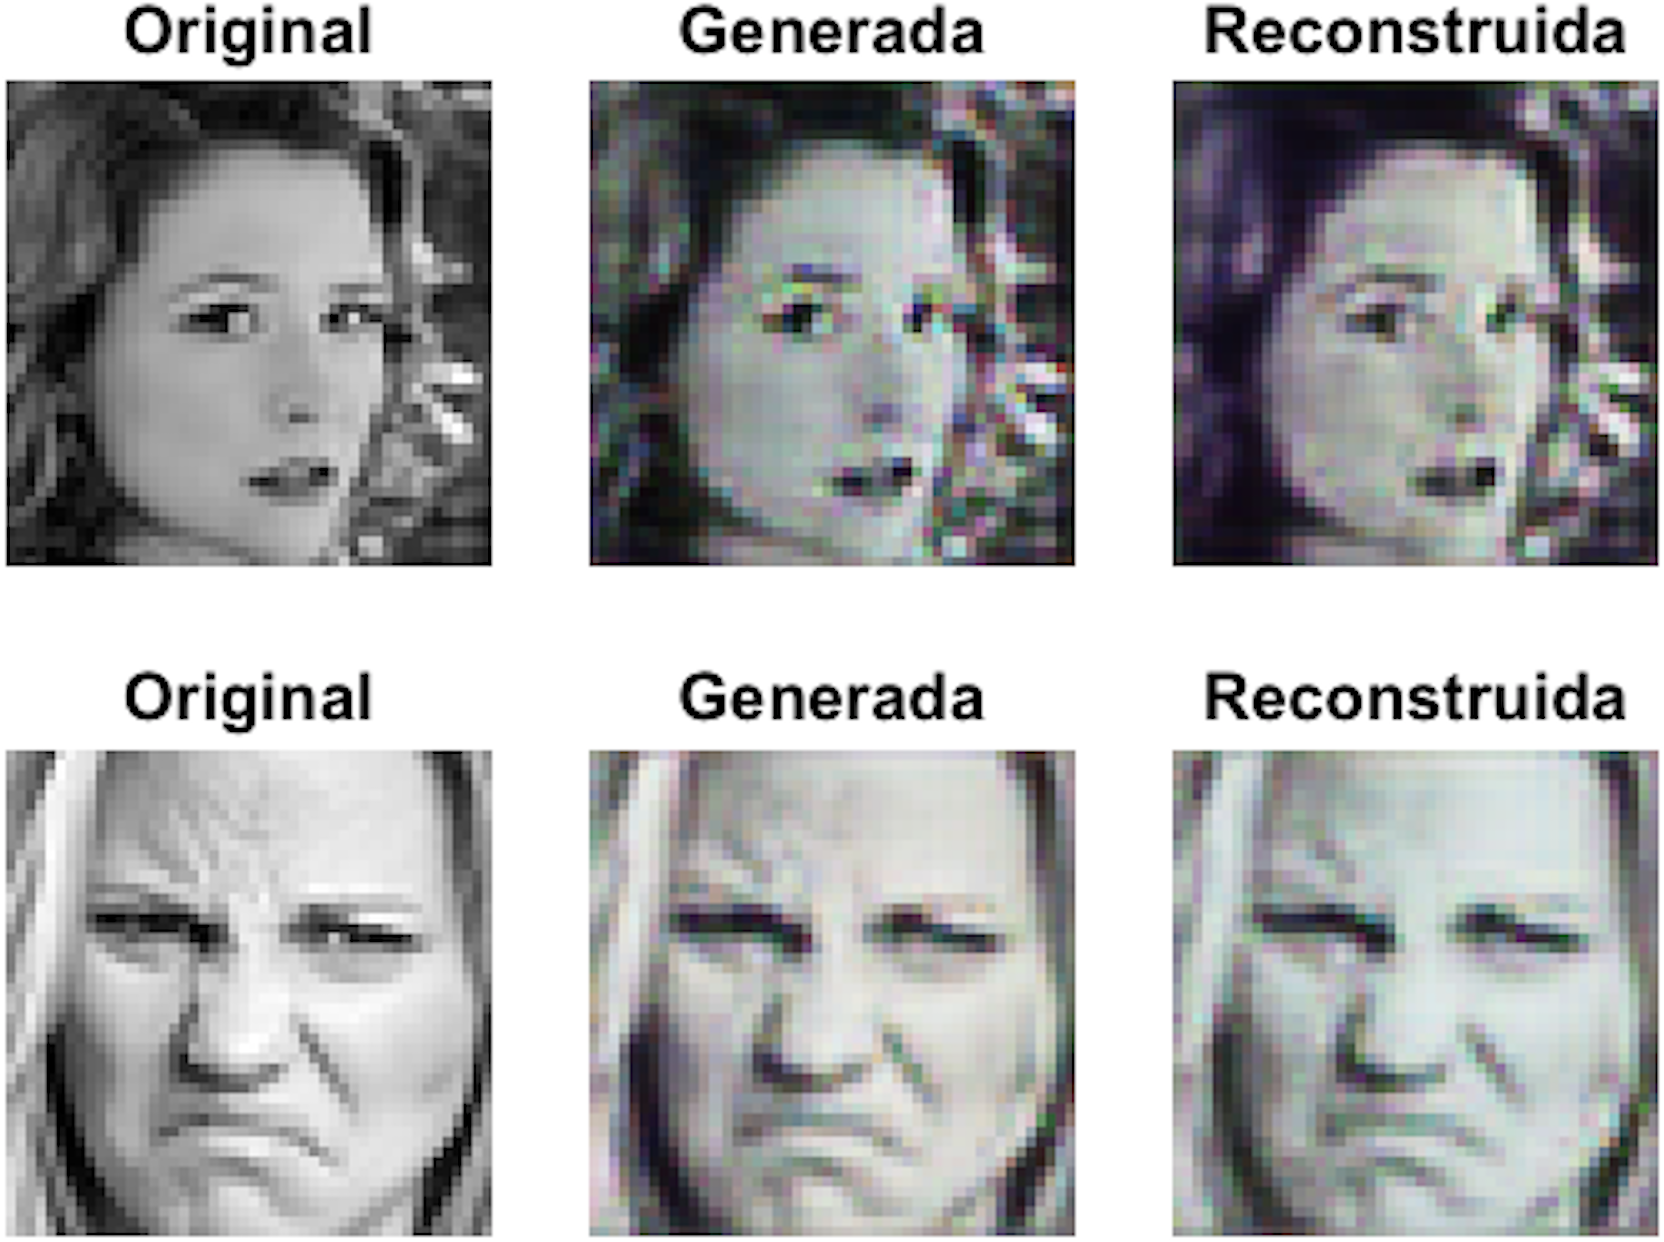
\includegraphics[width=\linewidth]{Images/CycleGAN_4000.png}
      \caption{Imágenes extraídas en la iteración $4\,000$.}
      \label{fig:CycleGAN_4000}
    \end{subfigure}
    \hfill
    \begin{subfigure}[t]{.45\textwidth}
      \centering
      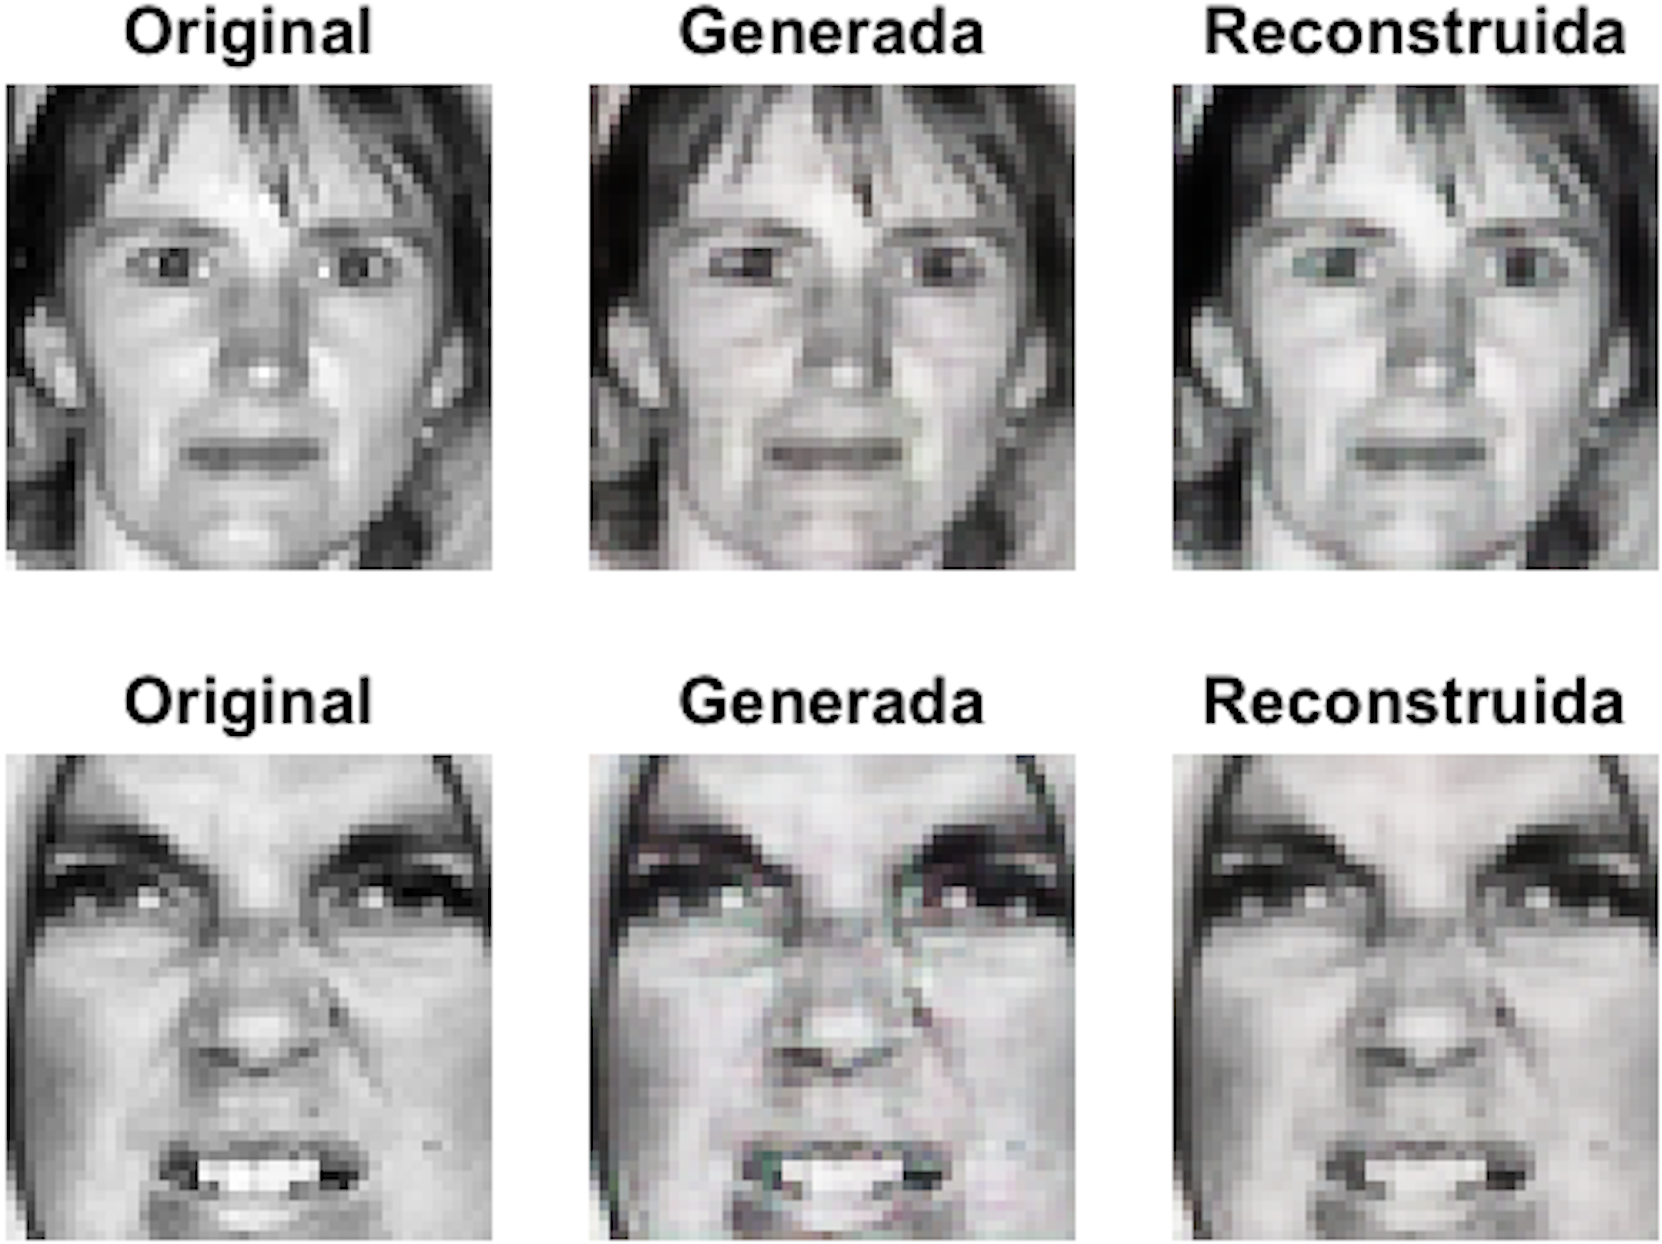
\includegraphics[width=\linewidth]{Images/CycleGAN_7300.png}
      \caption{Imágenes extraídas en la iteración $7\,300$.}
      \label{fig:CycleGAN_7300}
    \end{subfigure}
    \caption{Imágenes extraídas de la red CycleGAN durante el entrenamiento.}
    \label{fig:CycleGAN_images}
\end{figure}

Por otro lado, en la \autoref{fig:CycleGAN_images} se puede observar la progresión de unas determinadas imágenes a lo largo de este entrenamiento incompleto. Son visibles los indicios que muestran que la red progresa convenientemente, logrando apreciarse incluso en las últimas iteraciones (\autoref{fig:CycleGAN_7300}) la intensificación de la expresión neutral y un cierto suavizado en la expresión de asco.


    \chapter{Conclusiones y líneas futuras} \label{Chapter:7}


Por último, hace falta añadir que el código fuente de este trabajo está disponible, junto con los resultados y las instrucciones para replicarlos, en el siguiente repositorio: \url{https://github.com/ivadym/facial-expression-recognition}.
    \chapter{Conclusiones} \label{Chapter:8}

\section{Conclusiones}

A lo largo de este documento se han investigado y combinado algunas técnicas de visión por computador e inteligencia artificial para clasificar las expresiones faciales. Como se ha podido comprobar, este es un problema complejo que ha requerido de un análisis profundo para obtener unos resultados, que aunque no han sido los mejores, han alcanzado unos valores significativamente competitivos teniendo en cuenta el tiempo y los medios que se han invertido para afinar el modelo ResNet-50 pre-entrenado con la base de datos VGGFace2. En este contexto, la solución aquí planteada al problema del reconocimiento de expresiones faciales puede suponer una gran oportunidad para todos aquellos que deseen implementar un identificador de emociones con una respuesta más que aceptable y dispongan de recursos computacionales limitados.

De forma concreta, en un principio en este trabajo se propusieron dos puntos de vista desde los cuales abordar la tarea de identificaciones de emociones. Por un lado se han utilizado los modelos Inception-v3 e Inception-ResNet-v2 pre-entrenados sobre el conjunto ImageNet, mientras que por otro es empleada la red ResNet-50 preentrenada con la base de datos VGGFace2. A pesar de que objetivamente los dos primeros modelos han reportado mejores resultados en amplias tareas de aprendizaje profundo, el hecho de que ResNet-50 tenga los pesos adaptados al conjunto VGGFace2 marca la diferencia en favor de este último modelo. De hecho, las desigualdades reportadas son significativas, alcanzando el sistema ResNet-50 una precisión de $71.25\%$ sobre el conjunto de evaluación de la base de datos FER-2013, una tasa bastante superior a los $65.00\%$ y $63.86\%$ de las arquitecturas Inception-ResNet-v2 e Inception-v3 respectivamente. Esto evidencia la inmensa importancia que tiene la naturaleza de las imágenes empleadas en los modelos pre-entrenados. En realidad, el número y la calidad de los datos son fundamentales para obtener un buen desempeño, más incluso que el diseño de la propia arquitectura en algunas ocasiones, tal y como se ha podido comprobar a lo largo de este proyecto. Precisamente por este motivo es por el cual se ha decidido explorar la generación artificial de imágenes mediante las redes generativas antagónicas. Sin embargo, puesto que éstas son muy costosas de entrenar, finalmente no se ha podido llegar a unos resultados concluyentes al realizarse tan solo un entrenamiento parcial. A pesar de ello, hay numerosas evidencias empíricas que muestran que la aplicación de éstas técnicas de generación de datos pueden aumentar entre el 5\% y el 10\% el desempeño de los modelos iniciales \cite{GANAugmentation}, lo que en nuestro caso supondría la superación del estado del arte actual.

En última instancia también se ha logrado implementar un modelo de reconocimiento de expresiones faciales en tiempo real en un sistema empotrado, explorándose los servicios que este desarrollo sería capaz de ofrecer desde una perspectiva biomédica.

Finalmente, hace falta añadir que el código fuente de este trabajo está disponible, junto con los modelos entrenados, los resultados y las instrucciones para replicarlos, en el siguiente repositorio: \url{https://github.com/ivadym/FER}.

\section{Líneas Futuras}

Dada la multidisciplinariedad de este proyecto, hay una gran variedad de vías por las que seguir las investigaciones aquí plasmadas. De esta forma, por un lado sería interesante continuar con el objetivo inicial de diseño de un sistema de reconocimiento de expresiones faciales óptimo. En este contexto, podría resultar beneficioso realizar un entrenamiento de la red ResNet-50 completa y con una tasa de aprendizaje aún menor con el objetivo de obtener una mejor convergencia. Asimismo, también valdría la pena intentar terminar el entrenamiento incompleto de las redes CycleGAN, generar nuevas imágenes para la categoría correspondiente a la expresión de asco y comprobar si las mejoras que se obtienen son significativas. En caso de que lo fueran, es probable que la generación de más datos de las clases menos representadas pudiera dar lugar a que se superase el estado del arte actual.

Por otro lado y más en un contexto práctico, se podría enfocar la continuación de este proyecto a la obtención de un sistema de reconocimiento más heterogéneo, combinando varias bases de datos de expresiones faciales distintas. Esto tendría como objetivo mejorar el desempeño del reconocimiento en situaciones reales, en lugar de centrarse en obtener las mayores tasas sobre una base de datos determinada.

Esta última perspectiva es precisamente la que permitiría obtener un mejor funcionamiento del sistema implantado en el prototipo de espejo inteligente. Por ello, ésta es otra de las alternativas en las que se pueden enfocar los trabajos futuros: optimizar y añadir funcionalidades al espejo inteligente dentro del proyecto HOOP anteriormente descrito.

    \appendix
    \chapter{Impacto del Trabajo Fin de Grado}

\section{Impacto social}

\section{Impacto económico}

\section{Impacto medioambiental}

\section{Responsabilidad ética y profesional}

\clearpage
\newpage

    \chapter{Presupuesto económico del Trabajo Fin de Grado}

\clearpage
\newpage
    \chapter{Algoritmos} \label{Appendix:Algorithms}

\begin{algorithm}
\caption{Algoritmo de la retropropagación}
\label{alg:Backpropagation}
\begin{algorithmic}[1]
    \Function{Backpropagation}{datos, red}
        \State \VARIABLES pesos ($\omega_{i,j}$), tasa de aprendizaje ($\lambda$)
        \ForEach{$\omega_{i,j}$ \IN red} \Comment{Inicialización de parámetros}
            \State $\omega_{i,j} \gets$ pequeño valor aleatorio
        \EndFor
        \Repeat
            \ForEach{$x$ \IN datos} \Comment{Propagación de entradas\slash Obtención de salidas}
                \ForEach{neurona $j$ \IN capa i = 0} 
                    \State $\alpha_{0,j} \gets x$ \Comment{Asignación de las entradas}
                \EndFor
                \For{capa i = 1 \TO capa i = k}
                    \ForEach{neurona $j$ \IN capa i} 
                        \State $s_{i,j} \gets \sum\limits_{j} \omega_{i,j}\cdot \alpha_{i-1,j}$
                        \State $\alpha_{i,j} \gets f(s_{i,j})$ \Comment{Aplicación de la función de activación}
                    \EndFor
                \EndFor
                \ForEach{neurona $j$ \IN capa i = k} \Comment{Propagación hacia atrás}
                    \State $\Delta_{k,j} \gets f'(s_{k,j})\cdot (y_{k,j} - \alpha_{k,j})$ \textcolor{blue}{\footnotemark[1]}
                \EndFor
                \For{capa i = k-1 \TO capa i = 0}
                    \ForEach{neurona $j$ \IN capa i}
                        \State $\Delta_{i,j} \gets f'(s_{i,j})\cdot \sum\limits_{j} \omega_{i,j}\cdot \Delta_{i+1,j}$ \textcolor{blue}{\footnotemark[1]}
                    \EndFor
                \EndFor
                \ForEach{$\omega_{i,j}$ \IN red} \Comment{Actualización de los pesos}
                    \State $\omega_{i,j} \gets \omega_{i,j} - \lambda \cdot \alpha_{i,j} \cdot \Delta_{i,j}$ \Comment{Descenso Estocástico del Gradiente}
                \EndFor
            \EndFor
        \Until todos los datos se clasifican correctamente \OR satisfacción de otro criterio
        \State \Return red
    \EndFunction
\end{algorithmic}
\textcolor{blue}{\footnotesize{\\ $^1$ Conversión de la derivada de error con respecto a la salida en la derivada de error con respecto a la entrada multiplicándola por el gradiente de $f(s_{i,j})$.}}
\end{algorithm}

\begin{algorithm}
\caption{Algoritmo de la técnica de normalización por lotes \cite{BatchNormalization}}
\label{alg:BatchNormalization}
\begin{algorithmic}[1]
    \Function{BatchNormalization}{datos, red}
        \State \VARIABLES $\gamma, \beta$ \textcolor{blue}{\footnotemark[1]} \Comment{Parámetros por aprender}
        \Repeat
            \ForEach{lote $\mathfrak{B} = \lbrace x_{1 ... m}\rbrace$ \IN datos}
                \State $\mu_\mathfrak{B} \gets \frac{1}{m}\cdot \sum\limits_{i=1}^{m} x_i$ \Comment{Promedio del lote}
                \State $\sigma_\mathfrak{B}^{2} \gets \frac{1}{m}\cdot \sum\limits_{i=1}^{m} (x_i - \mu_\mathfrak{B})^2 $ \Comment{Varianza del lote}
                \State $\hat{x}_i \gets \frac{x_i - \mu_\mathfrak{B}}{\sqrt{\sigma_\mathfrak{B}^{2} + \epsilon}}$\Comment{Normalización}
                \State $y_i = \gamma \cdot \hat{x}_i + \beta$\Comment{Escalado y desplazamiento}
            \EndFor
        \Until todos los lotes de datos normalizados
        \State \Return $y$
    \EndFunction
\end{algorithmic}
\textcolor{blue}{\footnotesize{\\ $^1$ La tarea de los parámetros $ \gamma $ y $\beta$ es la de mantener la media y la varianza a unos valores preestablecidos.}}
\end{algorithm}
    \chapter{Figuras} \label{Appendix:Figures}

    \chapter{Miscelánea} \label{Appendix:Miscellaneous}

\begin{figure}
    \centering
    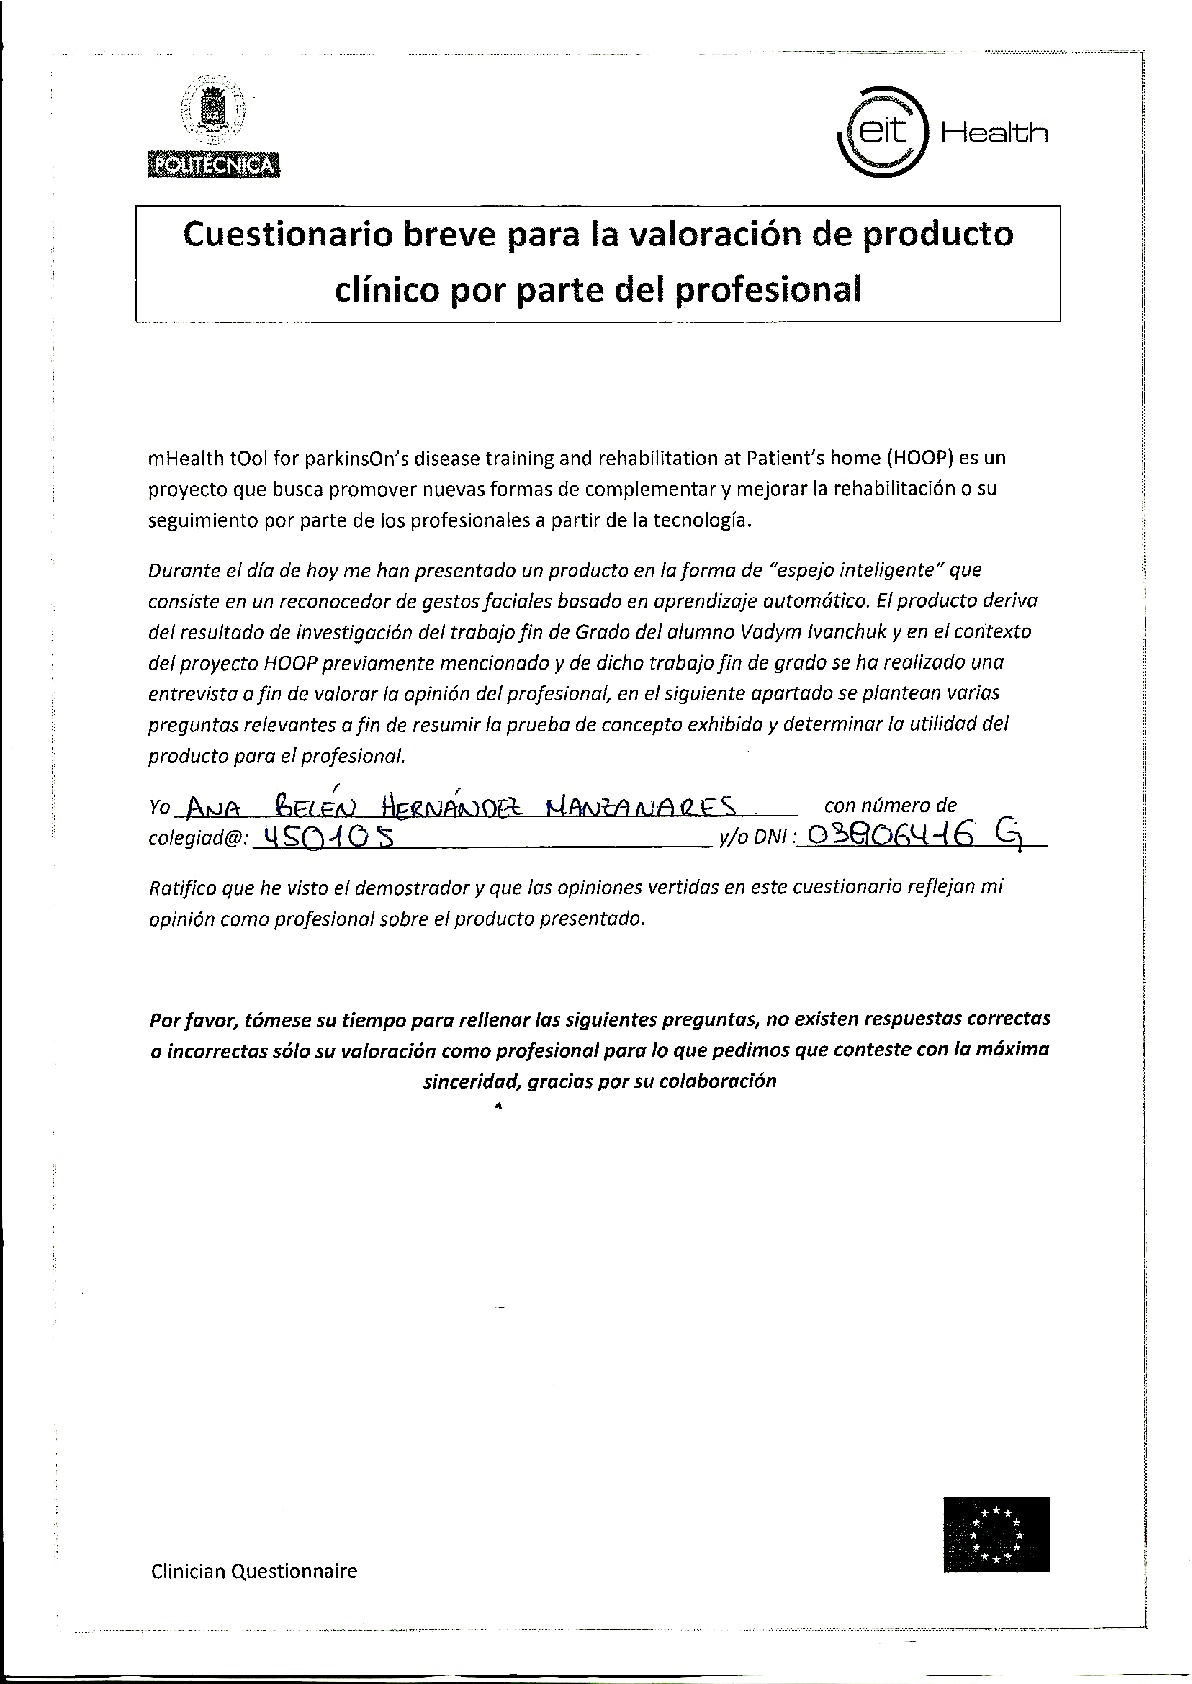
\includegraphics[width=\textwidth]{Images/informe_1.png}
    \caption{Informe reportado por la profesional de la AFA Parla.}
    \label{fig:Informe_1}
\end{figure}

\begin{figure}
    \centering
    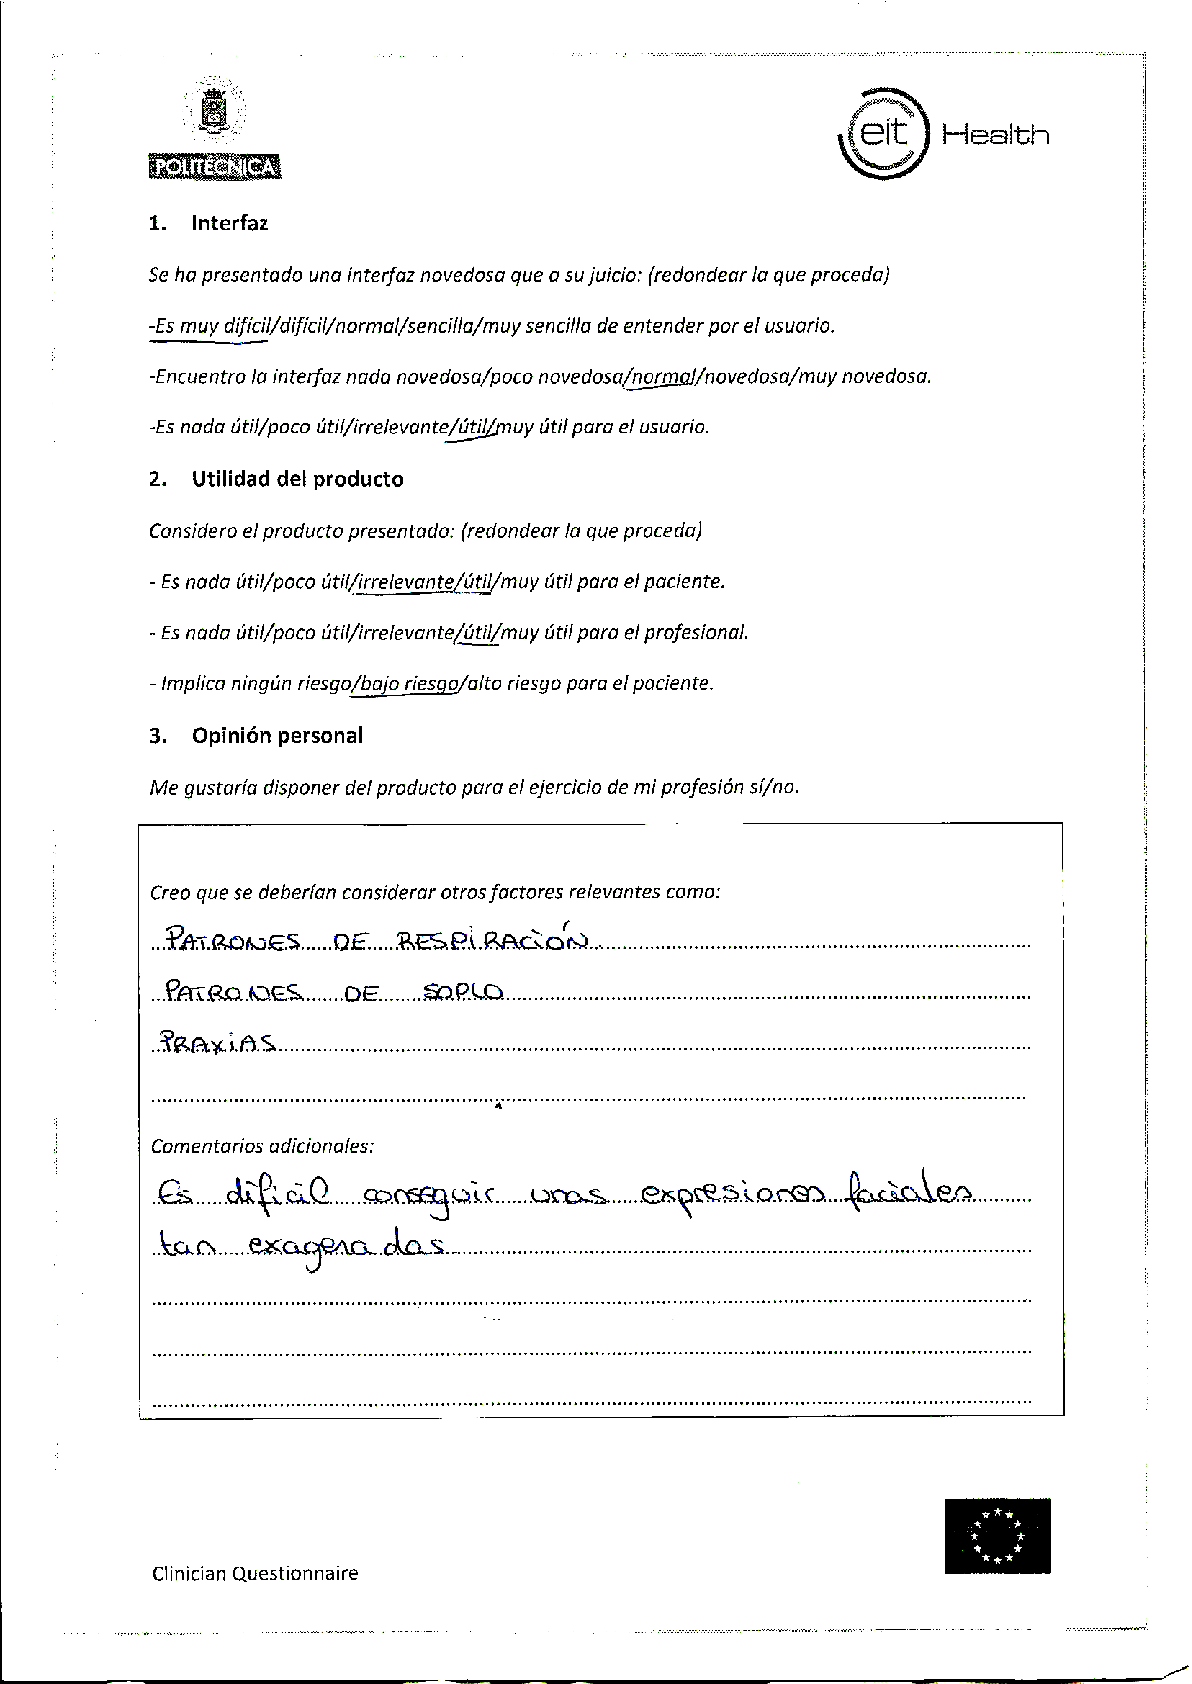
\includegraphics[width=\textwidth]{Images/informe_2.png}
    \caption{Informe reportado por la profesional de la AFA Parla.}
    \label{fig:Informe_2}
\end{figure}
    %% This defines the bibliography file (main.bib) and the bibliography style.
%% If you want to create a bibliography file by hand, change the contents of
%% this file to a `thebibliography' environment.  For more information 
%% see section 4.3 of the LaTeX manual.
\begin{singlespace}
\bibliography{Bibliography/main}
\bibliographystyle{plain}
\end{singlespace}
\end{document}